%%%%%%%%%%%%%%%%%%%%%%%%%%%%%%%%%%%%%%%%%
% Classicthesis Typographic Thesis
% LaTeX Template
% Version 1.4 (1/1/16)
%
% This template has been downloaded from:
% http://www.LaTeXTemplates.com
%
% Original author:
% André Miede (http://www.miede.de) with commenting modifications by:
% Vel (vel@LaTeXTemplates.com)
%
% License:
% GNU General Public License (v2)
%
% General Tips:
% 1) Make sure to edit the classicthesis-config.file
% 2) New enumeration (A., B., C., etc in small caps): \begin{aenumerate} \end{aenumerate}
% 3) For margin notes: \marginpar or \graffito{}
% 4) Do not use bold fonts in this style, it is designed around them
% 5) Use tables as in the examples
% 6) See classicthesis-preamble.sty for useful commands
%
%%%%%%%%%%%%%%%%%%%%%%%%%%%%%%%%%%%%%%%%%

%----------------------------------------------------------------------------------------
%	PACKAGES AND OTHER DOCUMENT CONFIGURATIONS
%----------------------------------------------------------------------------------------

\documentclass[
		titlepage,numbers=noenddot,headinclude,%1headlines,
	 	footinclude=true,
		dottedtoc, % Make page numbers in the table of contents flushed right with dots leading to them
		BCOR=0mm,paper=letter,fontsize=11pt, % Binding correction, paper type and font size
		american, % Languages, change this to your language(s)
		]{scrreprt} 
                
% Includes the file which contains all the document configurations and packages - make sure to edit this file
%%%%%%%%%%%%%%%%%%%%%%%%%%%%%%%%%%%%%%%%%
% Classicthesis Typographic Thesis
% Configuration File
%
% This file has been downloaded from:
% http://www.LaTeXTemplates.com
%
% Original author:
% André Miede (http://www.miede.de) with extensive commenting changes by:
% Vel (vel@LaTeXTemplates.com)
%
% License:
% GNU General Public License (v2)
%
% Important note:
% The main lines to change in this file are in the DOCUMENT VARIABLES
% section, the rest of the file is for advanced configuration.
%
%%%%%%%%%%%%%%%%%%%%%%%%%%%%%%%%%%%%%%%%%

%----------------------------------------------------------------------------------------
%	CHARACTER ENCODING
%----------------------------------------------------------------------------------------

\PassOptionsToPackage{utf8}{inputenc} % Set the encoding of your files. UTF-8 is the only sensible encoding nowadays. If you can't read äöüßáéçèê∂åëæƒÏ€ then change the encoding setting in your editor, not the line below. If your editor does not support utf8 use another editor!
\usepackage{inputenc}

%----------------------------------------------------------------------------------------
%	DOCUMENT VARIABLES
%	Fill in the lines below to enter your information into the thesis template
%	Each of the commands can be cited anywhere in the thesis
%----------------------------------------------------------------------------------------

% Remove drafting to get rid of the '[ Date - classicthesis version 4.0 ]' text at the bottom of every page
\PassOptionsToPackage{eulerchapternumbers,listings, pdfspacing, subfig,beramono,eulermath,parts}{classicthesis}
% Available options: drafting parts nochapters linedheaders eulerchapternumbers beramono eulermath pdfspacing minionprospacing tocaligned dottedtoc manychapters listings floatperchapter subfig

\newcommand{\myTitle}{Levelable Independence Complexes on Finite Simple Graphs\xspace}
\newcommand{\mySubtitle}{An Honours Integrated Science Thesis\xspace}
\newcommand{\myDegree}{\xspace}
\newcommand{\myName}{Michael Chong\xspace}
\newcommand{\mySupervisor}{Dr. Adam Van Tuyl\xspace}
\newcommand{\myFaculty}{Faculty of Science\xspace}
\newcommand{\myDepartment}{School of Interdisciplinary Science\xspace}
\newcommand{\myUni}{McMaster University\xspace}
\newcommand{\myLocation}{\xspace}
\newcommand{\myTime}{April 9, 2018\xspace}
\newcommand{\myVersion}{}

%----------------------------------------------------------------------------------------
%	USEFUL COMMANDS
%----------------------------------------------------------------------------------------

\newcommand{\ie}{i.\,e.}
\newcommand{\Ie}{I.\,e.}
\newcommand{\eg}{e.\,g.}
\newcommand{\Eg}{E.\,g.} 

\newcounter{dummy} % Necessary for correct hyperlinks (to index, bib, etc.)
\providecommand{\mLyX}{L\kern-.1667em\lower.25em\hbox{Y}\kern-.125emX\@}
\newlength{\abcd} % for ab..z string length calculation

%----------------------------------------------------------------------------------------
%	PACKAGES
%----------------------------------------------------------------------------------------

\usepackage{lipsum} % Used for inserting dummy 'Lorem ipsum' text into the template

%------------------------------------------------

%\PassOptionsToPackage{ngerman,american}{babel}  % Change this to your language(s)
% Spanish languages need extra options in order to work with this template
%\PassOptionsToPackage{spanish,es-lcroman}{babel}
\usepackage{babel}

%------------------------------------------------			

\usepackage{csquotes}
\PassOptionsToPackage{%
%backend=biber, % Instead of bibtex
backend=bibtex8,bibencoding=ascii,%
language=auto,%
style=numeric-comp,%
%style=authoryear-comp, % Author 1999, 2010
%bibstyle=authoryear,dashed=false, % dashed: substitute rep. author with ---
sorting=nyt, % name, year, title
maxbibnames=10, % default: 3, et al.
%backref=true,%
natbib=true % natbib compatibility mode (\citep and \citet still work)
}{biblatex}
\usepackage{biblatex}
 
 %------------------------------------------------

\PassOptionsToPackage{fleqn}{amsmath} % Math environments and more by the AMS 
 \usepackage{amsmath}
 
 %------------------------------------------------

\PassOptionsToPackage{T1}{fontenc} % T2A for cyrillics
\usepackage{fontenc}

%------------------------------------------------

\usepackage{textcomp} % Fix warning with missing font shapes

%------------------------------------------------

\usepackage{scrhack} % Fix warnings when using KOMA with listings package  

%------------------------------------------------

\usepackage{xspace} % To get the spacing after macros right

%------------------------------------------------

\usepackage{mparhack} % To get marginpar right

%------------------------------------------------

\PassOptionsToPackage{smaller}{acronym} % Include printonlyused in the first bracket to only show acronyms used in the text
\usepackage{acronym} % Nice macros for handling all acronyms in the thesis

%\renewcommand*{\acsfont}[1]{\textssc{#1}} % For MinionPro
\renewcommand*{\aclabelfont}[1]{\acsfont{#1}}

%------------------------------------------------

\PassOptionsToPackage{pdftex}{graphicx}
\usepackage{graphicx} 

%----------------------------------------------------------------------------------------
%	FLOATS: TABLES, FIGURES AND CAPTIONS SETUP
%----------------------------------------------------------------------------------------

\usepackage{tabularx} % Better tables
\setlength{\extrarowheight}{3pt} % Increase table row height
\newcommand{\tableheadline}[1]{\multicolumn{1}{c}{\spacedlowsmallcaps{#1}}}
\newcommand{\myfloatalign}{\centering} % To be used with each float for alignment
\usepackage{caption}
\captionsetup{font=small}
\usepackage{subfig}  



%----------------------------------------------------------------------------------------
%	HYPERREFERENCES
%----------------------------------------------------------------------------------------

\PassOptionsToPackage{pdftex,hyperfootnotes=false}{hyperref}
\usepackage{hyperref}  % backref linktocpage pagebackref
\pdfcompresslevel=9
\pdfadjustspacing=1

\hypersetup{
% Uncomment the line below to remove all links (to references, figures, tables, etc), useful for b/w printouts
%draft, 
colorlinks=true, linktocpage=true, pdfstartpage=3, pdfstartview=FitV,
% Uncomment the line below if you want to have black links (e.g. for printing black and white)
%colorlinks=false, linktocpage=false, pdfborder={0 0 0}, pdfstartpage=3, pdfstartview=FitV, 
breaklinks=true, pdfpagemode=UseNone, pageanchor=true, pdfpagemode=UseOutlines,%
plainpages=false, bookmarksnumbered, bookmarksopen=true, bookmarksopenlevel=1,%
hypertexnames=true, pdfhighlight=/O,%nesting=true,%frenchlinks,%
urlcolor=webbrown, linkcolor=RoyalBlue, citecolor=webgreen, %pagecolor=RoyalBlue,%
    %urlcolor=Black, linkcolor=Black, citecolor=Black, %pagecolor=Black,%
%------------------------------------------------
% PDF file meta-information
pdftitle={\myTitle},
pdfauthor={\textcopyright\ \myName, \myUni, \myFaculty},
pdfsubject={},
pdfkeywords={},
pdfcreator={pdfLaTeX},
pdfproducer={LaTeX with hyperref and classicthesis}
%------------------------------------------------
}

%----------------------------------------------------------------------------------------
%	AUTOREFERENCES SETUP
%	Redefines how references in text are prefaced for different 
%	languages (e.g. "Section 1.2" or "section 1.2")
%----------------------------------------------------------------------------------------

\makeatletter
\@ifpackageloaded{babel}
{
\addto\extrasamerican{
\renewcommand*{\figureautorefname}{Figure}
\renewcommand*{\tableautorefname}{Table}
\renewcommand*{\partautorefname}{Part}
\renewcommand*{\chapterautorefname}{Chapter}
\renewcommand*{\sectionautorefname}{Section}
\renewcommand*{\subsectionautorefname}{Section}
\renewcommand*{\subsubsectionautorefname}{Section}
}
\addto\extrasngerman{
\renewcommand*{\paragraphautorefname}{Absatz}
\renewcommand*{\subparagraphautorefname}{Unterabsatz}
\renewcommand*{\footnoteautorefname}{Fu\"snote}
\renewcommand*{\FancyVerbLineautorefname}{Zeile}
\renewcommand*{\theoremautorefname}{Theorem}
\renewcommand*{\appendixautorefname}{Anhang}
\renewcommand*{\equationautorefname}{Gleichung}
\renewcommand*{\itemautorefname}{Punkt}
}
\providecommand{\subfigureautorefname}{\figureautorefname} % Fix to getting autorefs for subfigures right
}{\relax}
\makeatother

%----------------------------------------------------------------------------------------

\usepackage{classicthesis} 

%----------------------------------------------------------------------------------------
%	CHANGING TEXT AREA 
%----------------------------------------------------------------------------------------

\linespread{1.05} % a bit more for Palatino
\areaset[current]{390pt}{761pt} % 686 (factor 2.2) + 33 head + 42 head \the\footskip
%\setlength{\marginparwidth}{7em}%
%\setlength{\marginparsep}{2em}%

%----------------------------------------------------------------------------------------
%	USING DIFFERENT FONTS
%----------------------------------------------------------------------------------------

%\usepackage[oldstylenums]{kpfonts} % oldstyle notextcomp
%\usepackage[osf]{libertine}
%\usepackage[light,condensed,math]{iwona}
%\renewcommand{\sfdefault}{iwona}
%\usepackage{lmodern} % <-- no osf support :-(
%\usepackage{cfr-lm} % 
%\usepackage[urw-garamond]{mathdesign} <-- no osf support :-(
%\usepackage[default,osfigures]{opensans} % scale=0.95 
%\usepackage[sfdefault]{FiraSans}


%% CUSTOMIZATION --------------------------------------------------------
% -----------------------------------------------------------------------

\usepackage{amsthm}
\usepackage{thmtools}
\usepackage{amssymb}
\usepackage{mathtools}
\newtheorem{theorem}{Theorem}[section]
\newtheorem{definition}[theorem]{Definition}
\let\olddefinition\definition
\renewcommand{\definition}{\olddefinition\normalfont}
\newtheorem{corollary}[theorem]{Corollary}
\newtheorem{lemma}[theorem]{Lemma}
\newcommand{\br}[1]{\{ #1 \}}
\newcommand{\ang}[1]{\langle #1 \rangle}
\newcommand{\ind}{\textrm{Ind}}
\newtheorem{example}[theorem]{Example}
\let\oldexample\example
\renewcommand{\example}{\oldexample\normalfont}
\newtheorem{question}{Question}[chapter]
\newtheorem*{question*}{Question}
%\renewcommand{\question}{\oldquestion\normalfont}
\newtheorem{conjecture}[question]{Conjecture}
%\renewcommand{\conjecture}{\oldconjecture\normalfont}
\newtheorem*{remark}{Remark}
\let\oldremark\remark
\renewcommand{\remark}{\oldremark\normalfont}


\newcommand{\changelocaltocdepth}[1]{%
  \addtocontents{toc}{\protect\setcounter{tocdepth}{#1}}%
  \setcounter{tocdepth}{#1}%
}

\usepackage{float}


\addbibresource{Bibliography.bib} % The file housing your bibliography
%\addbibresource[label=ownpubs]{Self_Publications.bib} % Uncomment for optional self-publications

%\hyphenation{Put special hyphenation here}

\begin{document}

\raggedbottom % Makes all pages the height of the text on that page

\selectlanguage{american} % Select your default language - e.g. american or ngerman

%\renewcommand*{\bibname}{new name} % Uncomment to change the name of the bibliography
%\setbibpreamble{} % Uncomment to include a preamble to the bibliography - some text before the reference list starts

\pagenumbering{roman} % Roman page numbering prior to the start of the thesis content (i, ii, iii, etc)

\pagestyle{plain} % Suppress headers for the pre-content pages

%----------------------------------------------------------------------------------------
%	PRE-CONTENT THESIS PAGES
%----------------------------------------------------------------------------------------

% Title Page

\begin{titlepage}

\begin{addmargin}[0cm]{0cm}
\begin{center}
\large

\hfill
\vfill

%\begingroup
\spacedallcaps{Levelable Simplicial Complexes} \\ \spacedallcaps{on Finite Simple Graphs} \\ \bigskip % Thesis title
%\endgroup

\spacedlowsmallcaps{\myName} \\  \medskip % Your name
\small\textit{supervised by} \\
\normalsize \spacedlowsmallcaps{\mySupervisor}

\vfill

\mySubtitle \\ \bigskip % Thesis subtitle
%\myDegree \\
\myDepartment \\
%\myFaculty
\myUni \\ \bigskip

\myTime

\vfill

\end{center}
\end{addmargin}

\end{titlepage} % Main title page

%\include{FrontBackMatter/Titleback} % Back of the title page

%\cleardoublepage\include{FrontBackMatter/Dedication} % Dedication page

%\cleardoublepage\include{FrontBackMatter/Foreword} % Uncomment and create a Foreword.tex to include a foreword

% Abstract

%\renewcommand{\abstractname}{Abstract} % Uncomment to change the name of the abstract

\pdfbookmark[1]{Abstract}{Abstract} % Bookmark name visible in a PDF viewer

\begingroup
\let\clearpage\relax
\let\cleardoublepage\relax
\let\cleardoublepage\relax

\chapter*{Abstract}
In commutative algebra, the Stanley-Reisner ideal allows for the construction of an artinian quotient ring (Stanley-Reisner ring) from a simplicial complex. Given some simplicial complex, it is sometimes possible to make a level artinian ring by adjoining powers of the variables as generators to the Stanley-Reisner ideal. In the cases where such a choice of powers exists, we call the simplicial complex “levelable". In this project, we discuss the case where the simplicial complex is the independence complex of a graph. That is, what graphs have an independence complex that can produce level rings through this construction? We investigate this question using a computer script in SageMath, and enumerate levelable graphs up to 10 vertices. We present families of graphs that satisfy and do not have the levelable property, and discuss graph operations that preserve and destroy this property.

\endgroup			

\vfill % Abstract page

%\cleardoublepage\include{FrontBackMatter/Publications} % Publications from the thesis page

\cleardoublepage% Acknowledgements

\pdfbookmark[1]{Acknowledgements}{Acknowledgements} % Bookmark name visible in a PDF viewer


\begingroup

\let\clearpage\relax
\let\cleardoublepage\relax
\let\cleardoublepage\relax

\chapter*{Acknowledgements}


My sincere thanks to my supervisor, Dr. Adam Van Tuyl, for his patience and guidance in this past year. Through this project he has enabled my growth as a mathematician, and I hope the text that follows reflects his exceptional teaching.

\bigskip
\noindent
I would also like to acknowledge my peers in the Integrated Science class of 2018 who have simultaneously been my colleagues, friends, and mentors at McMaster.

\bigskip
\noindent
To my friends in the Mathematics concentration, your acknowledgements are left as an exercise for the reader.
\endgroup
 % Acknowledgements page

\pagestyle{scrheadings} % Show chapter titles as headings

% Table of Contents - List of Tables/Figures/Listings and Acronyms

\refstepcounter{dummy}

\pdfbookmark[1]{\contentsname}{tableofcontents} % Bookmark name visible in a PDF viewer

\setcounter{tocdepth}{1} % Depth of sections to include in the table of contents - currently up to subsections

\setcounter{secnumdepth}{3} % Depth of sections to number in the text itself - currently up to subsubsections

\manualmark
\markboth{\spacedlowsmallcaps{\contentsname}}{\spacedlowsmallcaps{\contentsname}}
\tableofcontents 
\automark[section]{chapter}
\renewcommand{\chaptermark}[1]{\markboth{\spacedlowsmallcaps{#1}}{\spacedlowsmallcaps{#1}}}
\renewcommand{\sectionmark}[1]{\markright{\thesection\enspace\spacedlowsmallcaps{#1}}}

\clearpage

\begingroup 
\let\clearpage\relax
\let\cleardoublepage\relax
\let\cleardoublepage\relax

%----------------------------------------------------------------------------------------
%	List of Figures
%----------------------------------------------------------------------------------------


%----------------------------------------------------------------------------------------
%	List of Tables
%----------------------------------------------------------------------------------------

%----------------------------------------------------------------------------------------
%	List of Listings
%---------------------------------------------------------------------------------------- 

       
%----------------------------------------------------------------------------------------
%	Acronyms
%----------------------------------------------------------------------------------------
                   
\endgroup % Contents, list of figures/tables/listings and acronyms



\pagenumbering{arabic} % Arabic page numbering for thesis content (1, 2, 3, etc)
%\setcounter{page}{90} % Uncomment to manually start the page counter at an arbitrary value (for example if you wish to count the pre-content pages in the page count)
%----------------------------------------------------------------------------------------
%	THESIS CONTENT - CHAPTERS
%----------------------------------------------------------------------------------------
\include{Chapters/introduction} % Chapter 1

\cleardoublepage % Empty page before the start of the next part

%------------------------------------------------

\include{Chapters/definitions} % Chapter 2
% Chapter 1

\chapter{Introduction} % Chapter title

\label{ch:introduction} % For referencing the chapter elsewhere, use \autoref{ch:introduction} 

While combinatorics and commutative algebra have both long existed as independent mathematical disciplines, their applications to each other have only become apparent in recent decades. Richard Stanley, considered to be the father of the field of combinatorial commutative algebra, was among the first to connect commutative algebra techniques to combinatorial problems in his proof of the Upper Bound Conjecture for simplicial spheres in 1975 \cite{Stanley1975}. Soon after, in his influential 1977 paper \textit{Cohen-Macaulay complexes} \cite{Stanley1977}, Stanley first introduced the notion of a level algebra. Since then, level algebras have been an active area of research that has found applications in many other parts of mathematics. 

The goal of this thesis is to investigate a particular set of level rings that are constructed from the independence complexes of simple graphs. Rings arising from this construction are largely unexplored, and this project represents an initial step in addressing some of interesting questions in this area. We hope to thereby contribute to this new and evolving theory in commutative algebra.

The remaining chapters of this report follow this investigation. In \autoref{ch:background}, we start from elementary definitions of rings and ideals and develop the necessary background to understand the construction of artinian and level rings from the independence complex of a graph. Here we introduce our main research question: \textit{for what graphs does this construction allow for a level ring?} -- that is, \textit{what graphs are "levelable?"}. We approach this question using a criteria from Van Tuyl and Zanello \cite{VanTuyl2010} that reduces this question to checking for certain solutions to a specific linear system. In \autoref{ch:computer-results}, we describe how we applied this criteria in a computer search for levelable graphs on a small number of vertices. The data from this search was used to form hypotheses on the levelability of certain families of graphs. In \autoref{ch:levelable-results} we prove that certain families of graphs are levelable, and that certain graph operations preserve the levelable property. Then, in \autoref{ch:non-levelable-results} we present families of graphs that fail to be levelable, and graph operations that destroy the levelable property. Open questions and conjectures regarding this problem are listed in \autoref{ch:conjectures}. Finally, an atlas of levelable graphs is given in the \hyperref[ch:appendix]{Appendix}. 

% Chapter 2

\chapter{Definitions and Background} % Chapter title

\label{ch:background} % For referencing the chapter elsewhere, use \autoref{ch:examples} 

%-------------------------------------------------------------
This chapter introduces the necessary background to study levelable independence complexes. In \autoref{sec:ring-prelim}, we first introduce notation and elementary definitions in ring theory. In \autoref{sec:gradings}, we discuss what it means for a ring to be graded, and for a graded ring to be artinian and level. \autoref{sec:simplicial} and \ref{sec:levelable} discuss how artinian rings can be constructed from combinatorial objects called simplicial complexes, and a condition on simplicial complexes to determine when these artinian rings can be made level. \autoref{sec:bg-graphs} discusses a connection to graph theory, in which the simplicial complex is the independence complex of a graph. Finally, \autoref{sec:disconnected} introduces a prefatory result that will allow us to reduce our main question to connected graphs. 

\section{Preliminary definitions in ring theory} \label{sec:ring-prelim}

\subsection{Rings, ideals, and quotient rings} 

In abstract algebra \cite{Judson2016}, a \textbf{ring} $R$ consists of a set of elements with two binary operations, addition $(+)$ and multiplication $(\cdot)$, such that the following properties are satisfied for all elements $a$ and $b$ in $R$:
\begin{enumerate}
	\item $a + b = b + a$,
    \item $(a + b) + c = a + (b + c)$,
    \item there is some $0 \in R$ such that $a + 0 = a$ for all $a \in R$,
    \item for all $a \in R$, there is some $-a \in R$ such that $a + (-a) = 0$,
    \item $(ab)c = a(bc)$, and 
    \item $a(b+c) = ab + ac$, and $(a+b)c = ac + bc$.
\end{enumerate}
Additional properties allow us to define fields. A ring $R$ is a \textbf{field} if it also satisfies:
\begin{enumerate}
  \setcounter{enumi}{6}
  \item there is an element $1 \in R$ such that $1a = a1 = a$ for all $a \in R$, 
  \item $ab = ba$,
  \item if $ab = 0$, then $a = 0$ or $b = 0$, and
  \item for all $a \in R$, there exists an $a^{-1} \in R$ such that $aa^{-1} = a^{-1}a  = 1$.
\end{enumerate}
A \textbf{subring} $S$ of $R$ is a subset of elements of $R$ such that $S$ is also a ring under the same multiplication and addition operations of $R$. Of particular interest are ideals, which can be thought of as subrings with an ``absorbing'' property. An \textbf{ideal} $I$ in a ring $R$ is a subring of $R$ such that if $a \in I$ and $r \in R$, then $ar \in I$ and $ra \in I$. In alternative notation, $I$ is an ideal if for all $r \in R$, we have $rI \subseteq I$ and $Ir \subseteq I$ \cite{Judson2016}. 

If we have a ring $R$ and an ideal $I$ of $R$, we can construct a \textbf{quotient ring} $R/I$ as
$$
R/I= \br{r + I \; | \; r \in R}.
$$
A quotient ring is a ring under the addition and multiplication operations defined as follows:
\begin{gather*}
(a + I) + (b + I) =  (a + b) + I, \textrm{ and } \\
(a + I) (b + I) = (ab) I \textrm{.}
\end{gather*}


\subsection{Monomials, polynomials, and polynomial rings}

Given a set of variables $x_1, \dots, x_n$, we can define a \textbf{monomial} as a product of these variables of the form $x_1^{a_1} \cdots x_n^{a_n}$, where each of the exponents $a_1, \dots, a_n$ are non-negative integers. The sum of the exponents $a_1 + \cdots + a_n$ is called the \textbf{degree of the monomial}. We call a monomial \textbf{squarefree} if each of $a_1, \dots, a_n$ is either 0 or 1.

If $k$ is a field, then a \textbf{polynomial} $f$ in $x_1, \dots, x_n$ is a finite linear combination of monomials
$$
\sum_{i=1}^{m} r_i x_1^{a_{i_1}} \cdots x_n^{a_{i_n}} \, ,
$$
with coefficients $r_i$ in $k$. The set of all polynomials in $x_1, \dots , x_n$ with coefficients in $k$ is denoted $R = k[x_1, \dots, x_n]$. In fact, $R$ forms a ring called a \textbf{polynomial ring} \cite{Cox2007}. A polynomial $f$ in $k[x_1, \dots, x_n]$ is called a \textbf{homogeneous polynomial} if every monomial term in $f$ is of the same degree. 

As an example, we can take $k = \mathbb{Z}$, and take the polynomial ring in three indeterminates  $R = \mathbb{Z} [x, y, z]$. Then the polynomial $2xy^2 - 4y^3 + z^2z \in R$ is a homogeneous polynomial, since all of the monomial terms are of degree 3.

From this, we can define a \textbf{homogeneous ideal} as an ideal generated by homogeneous polynomials. That is, an ideal $I$ is homogeneous if 
$$
I = \br{g_1 f_1 + \dots +  g_sf_s \; |\; g_i \in R \,\textrm{and} \,  f_i \,\textrm{homogeneous for } i = 1, \dots, s}.
$$
We then call $\br{f_1, \dots, f_s}$ the \textbf{generators} of $I$, and write $I = \ang{f_1, \dots, f_s}$.

\section{Gradings and level algebras} \label{sec:gradings}

\subsection{Graded rings and ideals}
We call a ring $R$ \textbf{graded} if there exists a family of subgroups $\br{R_d}_{d \in \mathbb{Z}}$ of $R$ that satisfies the following properties:
\begin{enumerate}
	\item $R = \bigoplus\limits_{d \in \mathbb{N}} R_d$, and
    \item $R_i \cdot R_j \subseteq R_{i+j}$ for all $i, j \in \mathbb{Z}$.
\end{enumerate}

We can show that any polynomial ring $R$ is graded. Define $R_d$ to be all polynomials in $R$ with monomial terms of degree $d$. Since $R$ is all the polynomials with terms of any integer degree, $R$ is exactly the direct sum of all the $R_d$. Hence the first condition is satisfied. For the second criteria, consider some polynomial $f_i$ in $R_i$ and some polynomial $f_j$ in $R_j$. Then since all the monomial terms in $f_i$ are of degree $i$ and all the monomial terms in $f_j$ are of degree $j$, from multiplication of sums as usual (similar to the usual multiplication of polynomials over the real numbers) we have that the product $f_i \cdot f_j$ has only monomial terms of degree $i + j$. 

As an illustrative example of the second criteria, consider the polynomial ring $R = \mathbb{Q}[x, y, z]$. The polynomial $f = x^2 + 2yz$ is in $R_2$, since each monomial term $x^2$ and $2yz$ is of degree 2. Similarly, the polynomial $g = xy^2 + xyz$ is in $R_3$. Then we have that $f \cdot g = x^2 \cdot xy^2 + x^2 \cdot xyz + 2yz \cdot xy^2 + 2yz \cdot xyz \in R_{2+3} = R_5$, since every term is of degree 5. We would find this to be the case for any $f \in R_2$ and $g \in R_3$, and so $R_2 \cdot R_3 \subseteq R_{2+3} = R_5$.

Within a graded ring, we can have graded ideals. An ideal $I$ of a graded ring $R= \bigoplus  \limits_{d \in \mathbb{N}} R_d$ is called a \textbf{graded ideal} if we can write it as a direct sum of of the form $I = \bigoplus \limits_{d \in \mathbb{N}} (I \cap R_d)$. If $I$ is a graded ideal, then the associated quotient ring is also graded, and can be written:
$$
R/I = \bigoplus \limits_{d \in \mathbb{N}} R_d / I_d,
$$
where $I_n = I \cap R_n$. All homogeneous ideals $I = \ang{f_1, \dots, f_s}$ are graded. Consider some polynomial $p \in I$. Then $p = g_1 f_1 + \cdots + g_s f_s$, where each $g_i \in R$. Without loss of generality, we can assume that each $g_i$ is monomial (otherwise we can just expand the product of polynomials). Then each $g_i f_i$ is a the product of a monomial and a homogeneous polynomial, and $p$ is therefore a sum of homogeneous elements and $I$ is therefore graded.

A subclass of graded rings with particularly interesting properties are artinian algebras. There are several equivalent notions of artinian algebras. In our case, we will be use the following definition. A graded ring $R/I$ is an \textbf{artinian ring} if the Hilbert function of $R/I$ is eventually zero after a finite number of terms. The \textbf{Hilbert function} is defined as
$$
h(R/I) = (h_0, h_1, ...),
$$
where $h_i = \textrm{dim}_k (R/I)_i$ \cite{Stanley1978}. For a quotient ring $R/I$ with $I$ generated by monomials, we can think of $h_i$ simply as $\textrm{dim}_k (R_i) - \textrm{dim}_k(I_i)$, which is the number of monic monomials of degree $i$ in $R$ but not in $I$. Thus, for an artinian ring there is some integer $e$ with $h_i = 0$ for all $i > e$. Equivalently, we can define artinian quotient rings as follows: if $I$ is homogeneous and $R = k[x_1, \dots, x_n]$, then $R/I$ is artinian if and only if $\sqrt{I} = \ang{x_1, \dots, x_n}$. If a quotient ring $R/I$ is artinian, we can discuss its associated $h$-vector. The \textbf{$h$-vector} of an artinian quotient ring $R/I$ is just all the non-zero $h_i$ terms $(h_0, h_1, \dots, h_e)$ of its Hilbert function, where $h_i =0$ for all $i > e$. We call $e$ the \textbf{socle degree} of $R/I$. 

\subsection{Socles and level algebras} \label{sec:socles}
\label{socles-level}
We now introduce the socle of an artinian ring, which leads to the definition of a level algebra. The socle of an artinian (quotient) ring $R/I$, denoted $\textrm{soc}(R/I)$, is the set of all elements in $R/I$ such that multiplication with any monomial of degree 1 yields 0. So, if the grading of $R/I $ is given by $R/I = \bigoplus\limits_{d = 1}^{m-1} R_d / I_d$, and $x_i + I$ denotes an element of $(R/ I)_1$, then
$$
\textrm{soc}(R/I) = \br{F+I \in R/I \; | \; (F+I)(x_i + I) = 0 + I \textrm{ for all } i  = 1, ..., n}.
$$

\begin{lemma} 
$\textrm{soc}(R/I)$ is a homogeneous ideal of the artinian ring $R/I$.
\end{lemma}

\begin{proof} We will first use the ideal test to show that this is an ideal. Let $f + I$, $g+I \in \textrm{soc}(R/I)$. That is, $(f+I)(x_i + I) = (g+I) (x_i+I) = 0 + I$ for all $i$. 
Then $(f+I) - (g+I)  = (f-g) + I$, and 
$$
((f-g) + I)(x_i+I) = (f-g)x_i + I = (f x_i + I) - (g x_i + I) = 0 + I - 0 + I = 0 +I.
$$
Thus $(f+I) - (g+I) \in \textrm{soc} (R/I)$. 
Now let $p + I \in R/I$. Then $(p+I)(f+I) = pf + I$, and for any $x_i + I$, we have
$$
(pf + I) (x_i + I) = pfx_i + I = (p+I) (fx_i + I) = (p+I)(0+I) = 0+I.
$$
So $fp + I \in \textrm{soc} (R/I).$ Thus $\textrm{soc} (R/I)$ is an ideal of $R/I$. 

To show that $\textrm{soc}(R/I)$ is homogeneous, consider some $f+I \in \textrm{soc}(R/I)$. If we write $f+I = \sum_{d} f_d +I $ with $f_d+I \in (R/I)_d$, then we want that $f_d +I\in \textrm{soc}(R/I)$. If $f \in \textrm{soc}(R/I)$, then $f x_i +I = 0 + I$, but this would only happen if $f_d x_i +I$ for all $d$. Thus $f_d + I \in \textrm{soc} (R/I)$. 
\end{proof}

Since the socle is homogeneous, we can write it as the direct sum of homogeneous components. So $\textrm{soc}(R/I) = \textrm{soc}(R/I)_1 \oplus \, \textrm{soc}(R/I)_2 \oplus \, \dots $. For each homogeneous component $\textrm{soc}(R/I)_i$, we can denote with $s_i$ the dimension, in the field $k$, of the $i$\textsuperscript{th} homogeneous component. That is, let $s_i = \textrm{dim}_k \, \textrm{soc}(R/I)_i$. Note that if $I$ is a monomial ideal, then   $s_i = \textrm{dim}_k \textrm{soc} (R/I)_i $  is exactly the number of monic monomials $m$ of degree $i$ in $R \setminus I$ such that $mx_i \in $ I for $i = 1, \dots, n$.  We can then define the \textbf{socle-vector} $s(R/I)$ as the vector containing all such $s_i$, that is, $s(R/I) = (s_0, s_1, \dots, s_e)$.

If we compare the socle-vector of a quotient ring to its $h$-vector, we observe that $s_i \leq h_i$ for all $0 \leq i \leq e$. Since the socle of a ring is a subset of the ring itself, the dimension of the socle will never exceed that of ring. If we carry forward this result to the homogeneous components $R_i/I_i$ of a quotient ring $R/I = \bigoplus \limits_{d \in \mathbb{N}} R_d /I_d$, then we have that $s_i \leq h_i$ for all $i$. 

Finally, we can introduce the notion of a level algebra. We call $R/I$ a \textbf{level algebra of type $t$} if $s_0 = s_1 = s_2 = \cdots = s_{e-1} = 0$ and $s_e = h_e = t$, where $h_i = \textrm{dim}_k (R_i / I_i)$. That is, $R/I$ is level if its socle vector is of the form
$$
s(R/I) = (0, \dots, \, 0, t > 1) 
$$
In the special case where $t = 1$, $R/I$ is called \textbf{Gorenstein.}

\begin{example} Consider the polynomial ring $R = \mathbb{Q}[x, y]$, and the ideal $I = \ang{x^2, xy, y^2}$. First, we have that $R/I$ is artinian, since any monic monomial of degree $d \geq 3$ must be divisible by $x^2$, $xy$, or $y^2$. Now we consider the socle $\textrm{soc} (R/I)$ consisting of all the elements $f+I$ such that $f x + I = fy + I = 0 + I$. Notice that $\textrm{dim}(\textrm{soc} (R/I)_0) = 0$, since there are no monomials $m$ of degree 0 in $R \setminus I$ with $m x \in I$. However, $\textrm{dim}(\textrm{soc} (R/I)_1) = 2$, since there are two such monomials ($x$ and $y$) of degree 1. Indeed, $x \cdot x \in I$, $x \cdot y \in I$, and $y \cdot y \in I$. Thus $R/I$ is level of type 2.
\end{example}

\begin{example} Consider the same polynomial ring $R = \mathbb{Q}[x, y]$, and the ideal $I = \ang{x^2, xy^2, y^4}$. Again, $R/I$ is artinian since any monic monomial of degree $d \geq 4$ is divisible by at least one of the generators of the ideal. However, $R/I$ is not level. We have again that $\textrm{dim}(\textrm{soc}(R/I)_0) = 0$, since there are no monomials $m$ of degree 0 in $R \setminus I$ with $m y \in I$. Next, $\textrm{dim}(\textrm{soc}(R/I)_1) = 0$ since $xy \not \in I$, and so neither $x$ nor $y$ is in the socle. However, $\textrm{dim}(\textrm{soc}(R/I)_2) = 1$, since $xy \in R \setminus I$, $xyx \in I$ and $xyy \in I$. We also have that  $\textrm{dim}(\textrm{soc}(R/I)_3) \geq 1$, since $y^3 \in R \setminus I$,  $y^3 x \in I$, and $y^3 y \in I$. The socle vector therefore has at least two positive terms, and is therefore not level. 
\end{example}

\section{Level rings from simplicial complexes} \label{sec:simplicial}

\subsection{Simplicial complexes}
A simplicial complex $\Delta$ on a vertex set $S = \br{x_1, ..., x_n} $ is a collection of subsets of $S$ such that all singletons are elements of $\Delta$, and the simplicial complex is closed under taking subsets. That is, for any simplicial complex $\Delta$, we have:
\begin{enumerate}
	\item $\br{x_i} \in S$ for $i = 1, \dots, n$, and 
	\item if $X \in \Delta$ and $Y \subseteq X$, then $Y \in \Delta$. 
\end{enumerate} 
The elements of $\Delta$ are called \textbf{faces}, and those elements that are maximal under inclusion are called \textbf{facets}. For any facet $F$ and face $S$ of $\Delta$, if $F \subseteq S$ for some face $S \in \Delta$, then $F = S$. To simplifiy notation, we can write any simplicial complex as being generated by its facets. When we write $\Delta = \ang{ F_1, \dots, F_t }$, we mean that $\Delta$ consists of all subsets (proper and otherwise) of $F_1, \dots, F_t$. As an example, consider the simplicial complex 
$$
\Delta = \ang{ \br{x_2}, \br{x_1, x_3, x_4} }
$$
on the vertex set $V = \br{x_1, x_2, x_3, x_4}$.This is the same as writing 
$$
\Delta = \br{ \emptyset, \, \br{x_1}, \, \br{x_2}, \, \br{x_3},\,  \br{x_4}, \, \br{x_1, x_3}, \, \br{x_1, x_4},\, \br{x_3, x_4}, \, \br{x_1, x_3, x_4}}.
$$

\subsection{Stanley-Reisner ideals and rings}

Simplicial complexes can be associated with monomial ideals. Consider a polynomial ring $R = k[x_1, \dots, x_n]$, and a simplicial complex $\Delta$ on the vertex set $\br{x_1, \dots, x_n}$. The \textbf{Stanley-Reisner ideal} $I_\Delta$ on $R$ is the ideal generated by all squarefree monomials that correspond to the non-faces of $\Delta$, where a non-face is any subset of the vertex set not in $\Delta$. That is, 
$$
I_\Delta = \, \ang{x_{i_1} x_{i_2} \cdots x_{i_t} \; | \; \br{x_{i_1}, x_{i_2}, \dots, x_{i_t}} \not \in \Delta }.
$$
Some non-faces of $\Delta$ might be proper subsets of other non-faces, similar to how faces of $\Delta$ are subsets of its facets. Those non-faces that are minimal under inclusion of other non-faces are called \textbf{minimal non-faces}. Analogous to how we can write simplicial complexes as being generated by its facets, we can write $I_\Delta$ as being generated by the minimal non-faces: $I_\Delta = \ang{S_1, \dots, S_r}$.

Continuing with our above example, consider a polynomial ring on four variables $R = k[x_1, x_2, x_3, x_4]$, and the same simplicial complex as previous, $\Delta = \ang{ \br{x_2}, \br{x_1, x_3, x_4} }$. The corresponding Stanley-Reisner ideal is constructed by taking, as monomial generators, the subsets of vertices of $V$ that are not faces $\Delta$ to be generating elements. For instance, $x_2 x_4$ is an element of $I_\Delta$ since $\br{x_2, x_4}$ is not an element of $\Delta$. By taking all such sets, we have that 
$$
I_\Delta = \ang{x_1 x_2, \,  x_2 x_3, \, x_2 x_4}.
$$
Note that while $\br{x_2, x_3, x_4}$ is a non-face of $\Delta$, it is not a minimal non-face, since $\br{x_2, x_3}$ is also a non-face and $\br{x_2, x_3} \subset \br{x_2, x_3, x_4}$. We construct the corresponding \textbf{Stanley-Reisner ring} $R/I_\Delta$ by quotienting out the Stanley-Reisner ideal. 

\subsection{Construction of level rings from simplicial complexes}

We previously stated in \autoref{sec:socles} that a quotient ring $R/I$ is artinian if and only if $\sqrt{I} = \ang{x_1, \dots, x_n}$. Any Stanley-Reisner ring $R/I_\Delta$ is not a artinian algebra, except when $\Delta = \emptyset$ \cite{VanTuyl2010}. To see this, suppose for a contradiction that $\sqrt{I_\Delta} = \ang{x_1, \dots, x_n}$. Then for every $i$, there is some $a$ such that $x_i^a \in I_\Delta$. However, due to the way a Stanley-Reisner ideal is constructed, it is generated by squarefree monomials. It follows that if $x_i^a \in I_\Delta$ for some $a$, we must have $x_i \in I_\Delta$. Then since this is true for every $i$,  $I_\Delta = \ang{x_1, \dots, x_n}$, which forces $\Delta = \emptyset$. 

However, as noted in \cite{VanTuyl2010}, we can construct an algebra $A = A(\Delta, a_1, \dots, a_n)$ that \textit{is} artinian by adjoining powers of the variables to the ideal: 
$$
A = A(\Delta, a_1, \dots, a_n) : = R/\ang{I_\Delta, x_1^{a_1}, \dots,x_n^{a_n}}.
$$
As an example of such an artinian ring, consider the polynomial ring $R = k[x_1, x_2, x_3, x_4]$. On these variables, take the simplicial complex 
$$
\Delta = \ang{\br{x_1, x_2}, \br{x_2, x_4}, \br{x_3}}.
$$ 
The corresponding Stanley-Reisner ideal is 
$$
I_\Delta = \ang{x_1x_3, \, x_2x_3, \, x_3x_4,\,  x_4 x_1}.
$$
From this, we can construct a new ideal 
$$
J = \ang{I_\Delta, \, x_1^2,\,  x_2^2, \, x_3^2,\,  x_4^2} = \ang{x_1x_3, \, x_2x_3, \, x_3x_4,\,  x_4 x_1,  x_1^2,\, \allowbreak x_2^2, \, x_3^2,\,  x_4^2}.
$$ 
The associated quotient ring $R/J$ is artinian, and in fact level. To check this, recall from \autoref{socles-level} that an algebra $A$ is level of type $t$ if its socle-vector is of the form $s(A) = (0, 0, \dots, s_e = t)$. So, we need to calculate the components $s_i$ of the socle-vector. In the following, we will use the result that a monomial $m \in I$ if and only if there is a monomial generator of $I$ that divides $m$ \cite{Herzog2011}. 

\begin{enumerate}
	\item In order to calculate $s_0 = \textrm{dim}_k [\textrm{soc} (A) ]_0$, we are interested in the number of monic monomials $m$ of degree 0 not in $J$ such that $mx_i \in I$ for $i = 1, \dots, n$. However, there is only one monic monomial $m$ of degree 0 (that is, $m = 1$) and it does not count towards $s_0$, since $1 \cdot x_1 = x_1$ is not in the ideal $J$ (in fact, none of $x_1, \dots, x_n$ are in $J$). Thus, $s_0 = \textrm{dim}_k [\textrm{soc} (A) ]_0 = 0.$
	\item We have that $s_1 = \textrm{dim}_k[\textrm{soc} (A)]_1 = 0$ as well. This is because if we take any monic monomial $m$ of degree 1 (that is, take $m = x_1, \dots, x_n$) we notice that there is no $x_j$ that satisfies $x_jx_i \in J$ for all $J$.
    \item However, note that $s_2 = \textrm{dim}_k[\textrm{soc} (A) ] _ 2 > 0$. If we are only concerned about whether $R/J$ is level (and not the type), we only need to find one example of a degree 2 monomial $m \not \in J$ such that $mx_i \in J$ for $i = 1, \dots, n$. Indeed, taking $m = x_1x_3$ satisfies this condition. We can check multiplication with each of $x_1, \dots x_4$ individually:
    \begin{itemize}
    	\item Note that $mx_1 = (x_1x_3) x_1 = x_3 (x_1^2)$. Since $x_1^2$ is a generator of $J$, this is in $J$.
        \item Similarly, $mx_2 = (x_1 x_3) x_2 = x_1 (x_2 x_3) \in J$, since $x_2 x_3$ is a generator of $J$,
        \item $mx_3 = (x_1 x_3) x_3 = x_1 (x_3 ^2 )\in J$, since $x_3 ^2 $ is a generator of $J$, and
        \item $mx_4 = (x_1 x3) x_4 = x_1 (x_3 x_4) \in J$ since $x_3 x_4$ is a generator of $J$.
    \end{itemize}
    So $s_2 \geq 1$. 
	\item For any $s_l$ for $l \geq 3$, we have that $s_l = 0$. We can show this indirectly by showing that any monomial of degree 3 or greater must be in the ideal. We will show that any monomial $m$ of degree at least 3 can be absorbed into the ideal by choosing a degree 2 monomial $q$ that divides $m$. Consider the two following cases:
    \begin{itemize}
    	\item If the monomial is squarefree, then it contains at least three distinct choices of $x_1, \dots, x_4$. Therefore, it must be divisible by either $x_i x_{i+1}$ for some $i = 1, 2, 3$ or $x_4 x_1$. Since these are monomial generators of $J$, there is a monomial generator that divides $m$. Therefore $m$ must be in $J$.
        \item If the monomial is not squarefree, then at least one of the exponents of some $x_i$ in the monomial is or greater than or equal to 2. Then since $x_i^2$ is a generator of the monomial for $i = 1, 2, 3, 4$, we again have a monomial generator of $J$ that divides $m$. So $m$ is in $J$ in this case as well.
    \end{itemize}
    Thus $h_i = \textrm{dim}_k (R/J)_i = 0$ for all $i \geq 3$, and therefore $R/J$ is artinian. Furthermore, since $s(R/J) = (0, 0, t)$ with $t \geq 1$, we have shown that $R/J$ is also level.
\end{enumerate}

For algebras of the form $A(\Delta, a_1, \dots, a_n)$, we are only interested in cases in which $a_i \geq 2$ for all $i$. Van Tuyl and Zanello \cite{VanTuyl2010} point out that if some $a_i =1$, then
$$
A \cong k[x_1, \dots, \hat{x_i} , \dots , x_n] / (I_{\Delta '}, x_1^{a_i},\dots, \hat{x_i}, \dots , x_n^{a_n} ) = A(\Delta ' , x_1^{a_i},\dots, \hat{x_i}, \dots , x_n^{a_n} ),
$$
where $\Delta' $ is the same simplicial complex as $\Delta$ but with the faces containing $x_i$ omitted. That is, the face set of the simplicial complex $\Delta'$ is $\br{W \subseteq \Delta \, | \, W \subseteq V \setminus \br{x_i}}$. We can therefore assume that $a_i \geq 2$ in algebras of this form.

\section{Levelable simplicial complexes} \label{sec:levelable}

Given this construction of artinian rings, we are interested in what simplicial complexes $\Delta$ might yield an algebra $A = A(\Delta, a_1, \dots, a_n)$ that is level, and for what values of $(a_1, \dots, a_n)$ the algebra is level. Van Tuyl and Zanello \cite{VanTuyl2010} give a characterization of which such algebras are level by identifying a necessary and sufficient criteria on a particular linear system derived from the simplicial complex.

\begin{theorem}[Theorem 6 in \cite{VanTuyl2010}] \label{thm:level-condition} Let $\Delta$ be a simplicial complex on $n$ vertices with facets $\mathcal{F}(\Delta) = \br{F_1, \dots, F_t}$, where $t \geq 2$. Let $F_i = \br{x_{i,1}, \dots, x_{i, d_i}}$ denote the $i^{\textrm{th}}$ facet. Then the algebra $A(\Delta, a_1, \dots, a_n)$ with each $a_i \geq 2$ is level if and only if $(a_1, \dots, a_n)$ is a simultaneous integral solution to the following $t-1$ equations:

\begin{equation} \label{level-condition-eq}
\begin{aligned}
(x_{1, 1} + \cdots + x_{1, d_1}) - (x_{2, 1} + \cdots + x_{2, d_2}) &= d_1 - d_2 \\
(x_{2, 1} + \cdots + x_{2, d_2}) - (x_{3, 1} + \cdots + x_{3, d_3}) &= d_2 - d_3 \\
&\vdots \\
(x_{t-1, 1} + \cdots + x_{t-1, d_{t-1}}) - (x_{t, 1} + \cdots + x_{t, d_t}) &= d_{t-1} - d_t.
\end{aligned}
\end{equation}
\end{theorem}

From this condition, we define a \textbf{levelable} simplicial complex.
\begin{definition}
A simplicial complex $\Delta$ is \textbf{levelable} if there exists a tuple $(a_1, \dots, a_n)$, $a_i \geq 2$ for $i = 1, \dots, n$ such that the artinian algebra $A(\Delta, a_1, \dots, a_n)$ is level. That is, $\Delta$ is levelable if there exists solution to the linear system (\ref{level-condition-eq}). 
\end{definition}
To ease notation going forward, we define 
$$
S(X) := \sum_{x \in X} x
$$
so that the the $i^{\textrm{th}}$ equation in \eqref{level-condition-eq} can be written
$$
S(F_i) - S(F_{i+1}) = |F_i| - |F_{i+1}|.
$$
Some simplicial complexes can easily be identified as levelable. For instance, a simplicial complex is called \textbf{pure} if all its facets are the same size. In Mats Boij's Thesis \cite{Boij1994}, he gives the result that for a pure simplicial complex $\Delta$, then $A(\Delta, d, \dots, d)$ is level for every $d \geq 2$. We can arrive at this result using \autoref{thm:level-condition}. 

\begin{theorem}[Theorem 12(i) in \cite{VanTuyl2010}] \label{thm:pure} 
Let $\Delta$ be a simplicial complex on a vertex set on $n$ vertices with facets $\mathcal{F}(\Delta) = \br{F_1, \dots, F_t}$. If $|F_1| =  \cdots = |F_t| = \lambda$, then $\Delta$ is levelable.
\end{theorem}

\begin{proof}
Consider any equation $S(F_i) - S(F_{i+1}) = |F_i| - |F_{i+1}|$. If $|F_j| = \lambda$ for all $j$, then we can write this as $S(F_i) - S(F_{i+1}) = \lambda - \lambda = 0$. Now, if we set $x_1 = \cdots = x_n = d \geq 2$, then $S(F_i) - S(F_{i+1}) = \lambda d - \lambda d = 0$, thus satisfying any equation in \autoref{thm:level-condition}. Hence, the resulting algebra $A(\Delta, d, \dots, d)$ is level. Thus, pure simplicial complexes are always levelable, since a valid solution always exists.
\end{proof}

Van Tuyl and Zanello \cite{VanTuyl2010} also give the following result concerning simplicial complexes on small numbers of vertices.

\begin{theorem}[Theorem 12(ii) in \cite{VanTuyl2010}] \label{thm:small}
Any simplicial complex on $n \leq 4$ vertices is levelable. 
\end{theorem}

\autoref{thm:small} was obtained by checking all such simplicial complexes. In the same paper, simplicial forests, a class of complexes first introduced by Faridi \cite{Faridi2002}, are shown to be levelable. If $F$ is a facet of a simplicial complex $\Delta$, then $F$ is a \textbf{leaf} if $F$ is the only facet of $\Delta$, or there is some other facet $G \neq F$ of $\Delta$ such that for all facets $G' \neq F$ of $\Delta$, we have $G' \cap F \subseteq G \cap F$. In other words, leaves are those facets of $\Delta$ with a "stem" facet such that any intersection of any other facet with the leaf is contained in the intersection of the stem with the leaf. Then, we call $\Delta$ a \textbf{forest} if any simplicial complex $\Delta'$ generated by facets of $\Delta$ contains a leaf. 

Beyond these pioneering results, the question of which simplicial complexes are levelable is still an open question. One of the goals of this project is to study this problem by investigating a specific class of simplicial complexes arising from graphs.

\section{Graphs and independence complexes} \label{sec:bg-graphs}

Graph theory is a field of mathematics that can be related network structures. From graphs, we can construct algebraic objects and vice-versa. In this section, we discuss a connection between graph theory and algebra by using graphs -- in particular their independence complexes -- to construct Stanley-Reisner ideals $I_\Delta$ and subsequently, algebras of the form $A(\Delta, a_1 , \dots, a_n)$.

\subsection{Preliminary definitions}
In graph theory \cite{Wilson2010}, a \textbf{simple graph} $G=(V(G), E(G))$  consists of two sets: 

\begin{enumerate}
	\item the \textbf{vertex set}: a finite set $V(G) = \{ x_1, \dots , x_n \}$ of elements called \textbf{vertices}, and
	\item an \textbf{edge set}: a finite set $E(G)$ of distinct, unordered pairs $\{ x_i, x_j \}$ of distinct elements from $V(G)$, called \textbf{edges}.
\end{enumerate}

Vertices of graphs are commonly depicted as a collection of nodes $x_1, ... , x_n$, with lines drawn between two distinct nodes $x_i$ and $x_j$ if they share an edge; that is, if $\{x_i, x_j\} \in E(G)$. 

For a graph $G$, an \textbf{independent set} $W$ of $G$ is a subset of vertices of $G$ that do not share edges with each other. In other words, $x_i \in W$ and $x_j \in W$ if and only if $\br{x_i, x_j} \not \in E(G)$. Note that in this definition, any singleton $x_i$ of $V(G)$ is considered an independent set. We say that $W$ is a \textbf{maximal independent set}  of $G$ if it is not a proper subset of any other independent set of $G$. 

\subsection{Independence complexes as simplicial complexes}
From the notion of independent sets, we can define the \textbf{independence complex} of $G$, denoted $\ind(G)$, as the set of all independent sets of $G$. For any graph $G$, we can see that $\ind(G)$ is a simplicial complex. As noted previously, singleton sets $\br{x_i}$ are independent sets, and so $\br{x_i} \in \ind(G)$ for any $x_i \in V(G)$. Furthermore, $\ind(G)$ is closed under taking subsets. Consider some independent set $W = \br{x_{i_1}, \dots, x_{i_j}} \in \ind(G)$. No vertices in $W$ share an edge, and so if we take any any subset of vertices $X \subseteq W$, no elements of $X$ will share an edge either. The set $X$ is therefore an independent set of $G$ in itself, and so $X \in \ind(G)$. Therefore, the faces of $\ind(G)$ are all the independent sets of $G$, and it follows that the maximal independent sets are the facets of the simplicial complex $\ind(G)$, since these are maximal under inclusion. 

\begin{example} \label{ex:ind-set}
Consider the graph $G$ on 5 vertices with edge set 
$$
E(G) = \br{ \br{x_1, x_2}, \br{x_1, x_3}, \br{x_1, x_4}, \br{x_1, x_5}, \br{x_2, x_3}}.
$$ 
The independent sets of $G$, or the faces of $\ind(G)$ are 
\begin{equation*}
\begin{aligned}
\Delta = \ind(G) = \br{&\emptyset, \br{x_1}, \br{x_2}, \br{x_3}, \br{x_4}, \br{x_5},  \br{x_2, x_4}, \br{x_2, x_5}, \allowbreak \br{x_4, x_5}, \\ &\br{x_3, x_4}, \allowbreak \br{x_3, x_5}, \br{x_2, x_4, x_5}, \br{x_3, x_4, x_5}}.
\end{aligned}
\end{equation*}
However, every element of $\ind(G)$ is the subset of one of the following three maximal independent sets, or facets: $\br{x_1}$, $\br{x_2, x_4, x_5}$, or $\br{x_3, x_4, x_5}$.

\begin{figure}[bth]
    \myfloatalign
    \subfloat
    {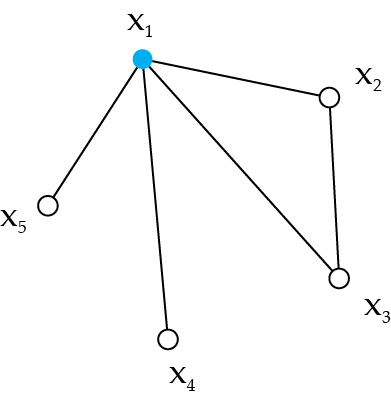
\includegraphics[width=.31\linewidth]{figures/ind-set1.png}} \quad
    \subfloat
    {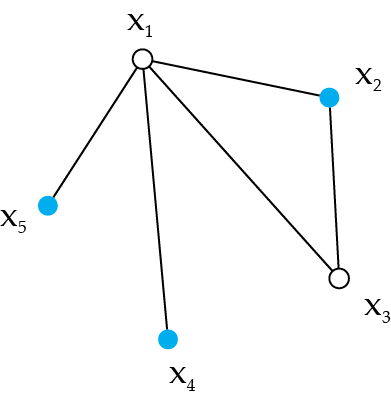
\includegraphics[width=.31\linewidth]{figures/ind-set2.png}} \quad
    \subfloat
    {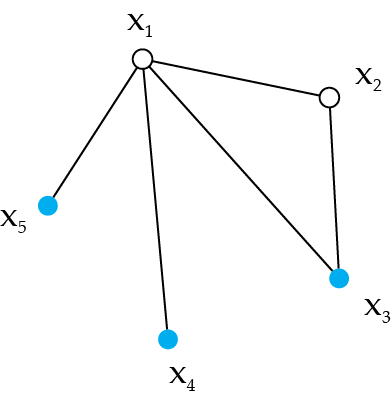
\includegraphics[width=.31\linewidth]{figures/ind-set3.png}} 
    \caption{Three copies of the graph $G$ in \autoref{ex:ind-set}. In each, one of the three maximal independent sets is highlighted in blue.}
\end{figure}
Since we have a simplicial complex, we can construct a Stanley-Reisner ideal that corresponds to the independence complex of $G$. From the way that $\ind (G)$ is constructed, the Stanley-Reisner is actually quite easy to describe. If $\Delta$ is the independence complex of some graph $G$, then its corresponding Stanley-Reisner ideal is that which is generated by monomials of the form $x_i x_j$, where $\br{x_i, x_j}$ is an edge of $G$. In more direct terms, since the faces of $\Delta = \ind (G)$ are exactly those subsets of $V(G)$ which do not share an edge, by definition the non-faces would be those subsets of $V(G)$ that do share an edge. This type of Stanley-Reisner ideal is called the \textbf{edge ideal} of $G$, denoted $I(G)$. That is, the ideal generated by the degree two squarefree monomials that correspond to an edge of $G$:
$$
I(G) := I_\Delta =  \ang{ x_i x_j \, |\, \br{x_i, x_j} \in E(G)}.
$$
Following through with our previous example yields the ideal
$$
I(G) = \ang{x_1 x_2,\,  x_1 x_3, \, x_1 x_4, \, x_1 x_5, \, x_2 x_3}.
$$
\end{example} 
Notice that we have a bijective correspondence between edge ideals in the polynomial ring in $n$ indeterminates $R = k[x_1, \dots, x_n]$ and simple graphs on $n$ vertices. The degree two squarefree monomials that generate the edge ideal uniquely define a graph on $n$ vertices, and vice-versa. 

Using the independence complex of a graph on $n$ vertices as a simplicial complex on the vertex set $\br{x_1, \dots, x_n}$ therefore allows us to construct artinian rings $A(\Delta, a_1, \dots, a_n)$, and there may exist certain choices of $(a_1, \dots, a_n)$ such that the resulting artinian ring is level. For the remainder of this report, we will investigate this special case in which the simplicial complex is the independence complex of a graph. In particular, we will explore the following question:

\begin{question*}
For what graphs $G$ is the independence complex $\Delta = \ind (G)$ levelable?
\end{question*}

Since each graph has a unique independence complex, we can think of levelability as a property of the graph, which gives us the following definition of a levelable graph.

\begin{definition}
A graph $G$ is \textbf{levelable} if its independence complex $\ind(G)$ is levelable. 
\end{definition}


\section{The levelable condition on disconnected graphs} \label{sec:disconnected}

In this section, we will show that the levelability of a graph depends entirely on the levelability of its connected components. That is, a graph is levelable if and only if its connected components are levelable.  This result drastically decreases the number of graphs that we need to check computationally, as well as reduces the problem of proving criteria. We begin by first defining graph connectedness.

\begin{definition}
Let $G$ be a graph on $n$ vertices $V(G) = \br{v_1, \dots, v_n}$. We call $G$ \textbf{connected} if, for every two vertices $v_i$, $v_j \in V(G)$ with $i \neq j$, there exists some sequence of edges $\br{v_i, v_{\alpha_1}}, \br{v_{\alpha_1}, v_{\alpha_2}}, \dots, \br{v_{\alpha_k}, v_j}$ that form a path connecting $v_i$ and $v_j$. A graph is \textbf{disconnected} if it is not connected. The \textbf{connected components} $G_1, \cdots G_m$ of $G$ are the maximal connected subgraphs of $G$. That is, each $G_i$ has vertex set $V(G_i) \subseteq V(G)$ such that every two distinct vertices in $V(G_i)$ are connected by a path, and there are no vertices in $V(G) \setminus V(G_i)$ that are adjacent to any vertex in $V(G_i)$. The edge set $E(G_i) \subset E(G)$ consists of all edges between vertices in $V(G_i)$.
\end{definition}

\begin{lemma} \label{lem:ind-sets-union}
Let $G = G_1 \cup G_2$ with $E(G_1) \cap E(G_2) = \emptyset$ and $V(G_1) \cap V(G_2) = \emptyset$. Let $\Delta_1$ denote $\ind(G_1)$, $\Delta_2$ denote $\ind(G_2)$, and $\Delta$ denote $\ind(G)$. If $S \in \Delta_1$ and $T \in \Delta_2$, then $S \cup T \in \Delta$.  
\end{lemma}

\begin{proof} We wish to show that if $v_i$, $v_j \in S \cup T$, then  $\{v_i, v_j\} \not \in E$. 

\noindent
\underline{Case 1}: $v_i \in S$ and $v_j \in S$.
Since $S \in \Delta_1$, it is an independent set, and so no vertices in $S$ share an edge. So $\{v_i, v_j\} \not \in E.$

\noindent
\underline{Case 2}: $v_i \in T$ and $v_j \in T$. 
Since $T \in \Delta_2$, it is an independent set, and so no vertices in $T$ share an edge. So $\{v_i, v_j\} \not \in E$.

\noindent
\underline{Case 3}: $v_i \in S$ and $v_j \in T$. 
If $v_i \in S$ and $v_j \in T$, then $v_i \in G_1$ and $v_j \in G_2$. Since $G_1$ and $G_2$ are disconnected, it must be that $\{ v_i, v_j \} \not \in E$.

Therefore no pair of vertices in $S \cup T$ share an edge, and $S \cup T \in \ind(G)$. 
\end{proof}

\begin{lemma} \label{lem:section-facets}
Suppose $G = G_1 \cup G_2$ with $E(G_1) \cap E(G_2) = \emptyset$ and $V(G_1) \cap V(G_2) = \emptyset$. Let $\Delta_1 = \ind(G_1)$, $\Delta_2 = \ind (G_2)$, and $\Delta = \ind (G)$. If $F(\Delta)$, $F(\Delta_1)$ and $F(\Delta_2)$ denote the facets of $\Delta$, $\Delta_1$ and $\Delta_2$ respectively, then $$F(\Delta) = \br{ F \cup H \, | \, F \in F(\Delta_1) , \, H \in F(\Delta_2)}.$$
\end{lemma}

\begin{proof}
Let $F \in F(\Delta_1)$ and $H \in F(\Delta_2)$. Then we need to show that any $F \cup H$ is an independent set in $\Delta$ that is maximal under inclusion.

First, notice that any element of $F(\Delta_1)$ or $F(\Delta_2)$ is an independent set in $\Delta$.
Therefore, by \autoref{lem:ind-sets-union} , $F \cup H \in \Delta$.

Now, we show that this is a maximal independent set; that is, if we take any additional vertex $v' \in G$ but $v' \not \in F \cup H$, then $F \cup H \cup \br{v'}$ fails to be an independent set.

Suppose for a contradiction that $F \cup H \cup \br{v'}$ was an independent set. Since $v' \in G$, either $v' \in G_1$ or $v' \in G_2$.  Without loss of generality, suppose $v' \in G_1$. By definition of the independent set, $v'$ does not share an edge with any vertex from $F \cup H$. In particular, it does not share any edges with any vertex in $F$. Then $F \cup \br{v'}$ is an independent set of $G_1$, and thus in $\Delta_1$.

We then have that $F \cup \{v'\} \in \Delta_1$ with $F \subsetneq F \cup \{v'\}$. But this contradicts $F$ being a facet of $\Delta_1$. So $F \cup H$ is a maximal independent set.

To see that these are the only facets of $\Delta$, consider some $F \in F(\Delta)$. We can express $F$ as a union of an independent set $S$ of vertices from $G_1$ and an independent set $T$ of vertices from $G_2$. Since $F$ is maximal, no vertex from $G = G_1 \cup G_2$ can be added to $F$ such that $F$ remains an independent set. 

That is, no vertex from $G_1$ can be added to $S$ so that $S$ is still an independent set, and no vertex from $G_2$ can be added to $T$ so that $T$ is still an independent set. Therefore $S$ and $T$ are maximal under inclusion, and are facets of $\Delta_1$ and $\Delta_2$ respectively.
\end{proof}

\begin{theorem} \label{thm:disconnected-1}
Suppose $G = G_1 \cup G_2$ with $E(G_1) \cap E(G_2) = \emptyset$ and $V(G_1) \cap V(G_2) = \emptyset$. Then $\Delta = \ind(G)$ is levelable if and only if $\Delta_1 = \ind(G_1)$ and $\Delta_2 = \ind(G_2)$ are both levelable.
\end{theorem}


\begin{proof}
We will first assume that both $\Delta_1$ and $\Delta_2$ are levelable, and prove that $\Delta$ must also be levelable.

Suppose component $G_1$ is a graph on $\alpha$ vertices, and $G_2$ is a graph on $\beta$ vertices. Then $G$ is a graph on $\alpha + \beta$ vertices. Let us the label the vertices of $G$ as $\{ x_1 , \dots , x_\alpha, y_{1} , \dots , y_{\beta} \}$, where the first $\alpha$ vertices are from $G_1$ and the latter $\beta$ are from $G_2$. 

If $F(\Delta_1) = \{ F_1, \dots , \, F_M \}$, and $\Delta_1$ is levelable, then there exists some solution $(a_1, \dots , a_\alpha)$, with $\alpha_i \in \mathbb{Z}$, $a_i \geq 2$ to the following system of $M-1$ equations:
\begin{equation}
\label{eq:G1system}
  \begin{aligned}
	S(F_1) - S(F_2) & = |F_1| - |F_2| \\
	S(F_2) - S(F_3) & = |F_2| - |F_3|\\
	&\vdots \\
	S(F_{M-1}) - S(F_M) & = |F_{M-1}| - |F_{M}|.
  \end{aligned}
\end{equation}
If $F(\Delta_2) = \{ H_{1}, \dots , \, H_N \}$, and $\Delta_2$ is levelable, then there exists some solution $(b_1, \dots , b_\beta)$, with $b_i \in \mathbb{Z}$, $b_i \geq 2$ to the following system of $N-1$ equations:
\begin{equation}
\label{eq:G2system}
  \begin{aligned}
	S(H_1) - S(H_2) & = |H_1| - |H_2| \\
	S(H_2) - S(H_3) & = |H_2| - |H_3|\\
	&\vdots \\
    S(H_{N-1}) - S(H_N)& = |H_{N-1}| - |H_N|.
  \end{aligned}
\end{equation}
By \autoref{lem:section-facets}, we have that $F(\Delta) = \{ F_i \cup H_j \, | \,  1 \leq i \leq M , \, 1 \leq j \leq N \}$. Let us label the elements $K_l$ of $F(\Delta)$ as follows:
\begin{equation} \label{all-facets}
\begin{aligned}
	K_1 &= F_1 \cup H_1 \\
    K_2 &= F_1 \cup H_2 \\
    & \; \vdots \\
    K_{N-1} &= F_1 \cup H_{N-1} \\
    K_N &= F_1 \cup H_N \\
    K_{N+1} &= F_2 \cup H_N \\
    & \; \vdots \\ 
    K_{2N-1} &= F_{2} \cup H_{2} \\
	K_{2N} &= F_{2} \cup H_{1} \\
    K_{2N+1} &= F_{3} \cup H_{1} \\
    & \; \vdots \\
    K_{MN-1} &= F_{M} \cup H_{N-1} \\
    K_{MN} &= F_{M} \cup H_{N}. \\
\end{aligned}
\end{equation}
Now, $\Delta$ is levelable if there is some solution $(z_1, \dots , z_{\alpha + \beta})$ of the following system of $MN - 1$ equations:
\begin{equation}
\label{eq:Gsystem}
  \begin{aligned}
	S(K_1) - S(K_2) & = |K_1| - |K_2| \\
	S(K_2) - S(K_3) & = |K_2| - |K_3| \\
	&\vdots \\
	S(K_{MN - 1}) - S(K_{MN}) x & = |K_{MN-1}| - |K_{MN}|.
  \end{aligned}
\end{equation}
We will show that $(a_1, \dots , a_\alpha,  b_1, \dots,b_\beta)$ is a solution to the system of equations \eqref{eq:Gsystem}. Consider the $t^{\textrm{th}}$ equation in the system $S(K_t) - S(K_{t+1}) = |K_t| - |K_{t+1}|$. \\

\noindent
\underline{Case 1:} $t$ is not a multiple of N. Then we can write $K_t$ and $K_{t+1}$ as either
\begin{equation} \label{eq:K1}
\begin{aligned}
K_t = F_i \cup H_j \; \textrm{and} \; K_{t+1} = K_i \cup H_{j+1}
\end{aligned}
\end{equation}
or
\begin{equation} \label{eq:K2}
\begin{aligned}
K_t = F_i \cup H_j \; \textrm{and} \; K_{t+1} = K_i \cup H_{j-1}.
\end{aligned}
\end{equation}
In the case of \eqref{eq:K1}, the $t^{\textrm{th}}$ equation can be written as
$$
S(F_i \cup H_j) - S(F_i \cup H_{j+1}) = | F_{i} \cup H_{j}| - | F_{i} \cup H_{j+1}|.
$$
Since $F_{i}$ is necessarily disjoint from $H_{j}$ and $H_{j+1}$, we can rewrite this as:
\begin{equation*}
\begin{aligned}
S(F_i) + S(H_j) - S(F_i) - S(H_{j+1}) &=  |F_i| + | H_{j}| - |F_i| - |H_{j+1}|,
\end{aligned}
\end{equation*}
which reduces to
\begin{equation*}
\begin{aligned}
S(H_j) - S(H_{j+1}) &=  | H_{j}| - |H_{j+1}|.
\end{aligned}
\end{equation*}
The resulting equation depends only on vertices from $G_2$ (in particular, it is the $j^{\textrm{th}}$ equation in \eqref{eq:G2system}). Thus $(a_1, \dots, a_\alpha, b_1, \dots, b_\beta)$ is a solution to this equation. 

In the case of \eqref{eq:K2}, the $t^{\textrm{th}}$ equation can be written:
\begin{equation*}
\begin{aligned}
S(F_{i} \cup H_{j}) - S(F_{i} \cup H_{j-1}) = | F_{i} \cup H_{j}| - | F_{i} \cup H_{j-1}|.
\end{aligned}
\end{equation*}
Multiplying by $-1$ yields
$$
S(F_{i} \cup H_{j-1}) - S(F_{i} \cup H_{j}) = | F_{i} \cup H_{j-1}| - | F_{i} \cup H_{j}|.
$$
Again, since $F_i$ is disjoint from $H_{j-1}$ and $H_j$, we can write this as 
\begin{equation*}
\begin{aligned}
S(F_i) + S(H_{j-1}) - S(F_i) - S(H_{j}) &=  |F_i| + | H_{j-1}| - |F_i| - |H_{j}|,
\end{aligned}
\end{equation*}
which reduces to
\begin{equation*}
\begin{aligned}
S(H_{j-1}) - S(H_{j}) &= | H_{j-1}| - |H_{j}|.
\end{aligned}
\end{equation*}
This is the $(j-1)^{\textrm{th}}$ equation in \eqref{eq:G2system}, and thus $(a_1, \dots a_\alpha, b_1, \dots , b_\beta)$ is a solution to this equation, since it only depends on the vertices from $G_2$. \\

\noindent
\underline{Case 2}: $t$ is a multiple of $N$. Then 
$$
K_t = F_i \cup H_j \; \textrm{and} \; K_{t+1} = F_{i+1} \cup H_j,
$$
where either $j=1$ or $j=N$. The $t^{\textrm{th}}$ equation can therefore be written
\begin{equation} \label{eq:N}
\begin{aligned}
S(F_{i} \cup H_{j}) - S(F_{ i+1} \cup H_{j}) = | F_{i} \cup H_{j}| - |F_{i+1} \cup H_{j}|,
\end{aligned}
\end{equation}
and since $H_j$ is disjoint from $F_i$ and $F_{i+1}$, we can write this as
\begin{equation*}
\begin{aligned}
S(F_{i}) + S(H_{j}) -  S(F_{i+1})  -S(H_{j})  &= | F_{i} | + | H_{j}| - | F_{i+1}| - |H_{j}|.
\end{aligned}
\end{equation*}
This reduces to
\begin{equation*}
\begin{aligned}
S(F_{i})-   S(F_{i+1})   &= | F_{i} | - | F_{i+1}|,
\end{aligned}
\end{equation*}
which is the $i^{\textrm{th}}$ equation in \eqref{eq:G1system} and concerns only the $\alpha$ vertices from $G_1$, and so we have that $(a_1, \dots, a_\alpha, b_1, \dots,  b_\beta)$ is a solution to the equation.

We then have that $(a_1, \dots, a_\alpha, b_1, \dots, b_\beta)$ is a simultaneous solution to the system of equations \eqref{eq:Gsystem}, and $\Delta$ is levelable. \\


Now, we prove the other direction. That is, if $\Delta_1$ or $\Delta_2$ fail to be levelable, then $\Delta$ is also not levelable. Without loss of generality, assume that $\Delta_1$ is not levelable. Label the facets of $\Delta$ as in \eqref{all-facets}. If we consider every $t^{\textrm{th}}$ equation where $t$ is a multiple of $N$, similar to \eqref{eq:N} we can reduce each equation to the form
\begin{equation}
\begin{aligned}
S(F_i) - S(F_{i+1}) = |F_i| - |F_{i+1}|. 
\end{aligned}
\end{equation}
Applying this to every $N^{\textrm{th}}$ equation in system \eqref{eq:Gsystem} returns the $M-1$ equations in \eqref{eq:G1system} which depends exclusively on vertices in $G_1$. Since $\Delta_1$ is assumed to fail to be levelable, there is no valid choice of $(a_1, \dots, a_\alpha)$ that simultaneously satisfies these $M-1$ equations, and there is therefore no simultaneous solution to the system of $MN-1$ equations. Therefore $G$ is not levelable. 
\end{proof}

\begin{theorem} \label{thm:disconnected-iff}
Let $G$ a graph with connected components $G_1, \dots, G_m$. Then $G$ is levelable if and only if each of its individual connected components are levelable.
\end{theorem}

\begin{proof}
Suppose that $G$ is levelable. For any $i$, $G \setminus G_i$ and $G_i$ satisfy the condition for $G_1$ and $G_2$ in \autoref{thm:disconnected-1}. Therefore $G_i$ must be levelable. Since the choice of $i$ was arbitrary, each of $G_1, \dots, G_m$ is individually levelable.

Now suppose that each of $G_1$ is levelable. Define $H_k = \bigcup_{i = 1}^k G_i$. We will show that $G$ is levelable by an induction argument. The base case is true since $H_1 = G_1$ is levelable by assumption. For the induction step, suppose that $H_{k-1}$ is levelable. Then $H_k = H_{k-1} \cup G_k$ is levelable by \autoref{thm:disconnected-1}, since $G_k$ is levelable.

Therefore $H_k$ is levelable for $i = 1, \dots, m$. In particular, $H_m = G_1 \cup \cdots \cup G_m = G$ is levelable, as required.
\end{proof}

\autoref{thm:disconnected-iff} tells us that the levelability of disconneted graphs depends completely on the levelability on all of its connected components. Therefore, for the rest of this document we will consider only connected graphs, keeping in mind that all these results can easily be extended to all simple graphs.
\chapter{Computer Methods and Results}
\label{ch:computer-results}

In order to guide our investigation of the levelability of graphs, we used computational tools to check for the existence of valid solutions to \autoref{thm:level-condition} on graphs on small numbers of vertices. In particular, a computer script was written using SageMath to check all connected graphs on 10 or fewer vertices.

\section{Data generation}
Using the convenient built-in capabilities of SageMath, we applied \autoref{thm:level-condition} to determine levelability on all connected graphs on 10 or fewer vertices. Graphs were generated using the \texttt{graphs.nauty\_geng()} generator object in SageMath. The $t$ maximal independent sets for each graph \texttt{G} were extracted using the function \texttt{IndependentSets(G, maximal = True)}, and the corresponding linear system was constructed as a matrix with $t-1$ rows and $n$ columns. The existence of integer solutions to \autoref{thm:level-condition} with the $x_i \geq 2$ constraint were checked using \texttt{MixedIntegerLinearProgram()}: a built-in linear program function in SageMath. The solution to the system, if one was returned by the linear program, was checked against the original system to verify the solution. If the linear program failed to return a solution, the graph was determined to not be levelable. 

One challenge in recording these data is that graphs do not have unique vertex labellings. Therefore, the graph object generated by \texttt{graphs.nauty\_geng()} may not be the same ``object" as an isomorphic, but differently labelled graph. Therefore, before recording data, each generated graph object was transformed to a unique ``canonical" label using \texttt{canonical\_label()}. If we were to then generate an isomorphism of some graph in another analysis, we can reduce it to the canonical label to match our data set to avoid miscommunication and confusion. The graph6 string for each (canonically labelled) graph was saved in a data frame along with a boolean variable (\texttt{1} if levelable or \texttt{0} if not). The source code and data for this project is available at \url{https://github.com/michael-chong/levelable}. Psuedocode for the data generation is outlined in  \autoref{lst:pseudocode}.

\begin{lstlisting}[mathescape = true, float=bthp,frame=tb,caption={Data generation pseudocode},label=lst:pseudocode]
for n = 4,...,10:
  
  DF = data frame to hold results
  
  for each connected graph G on n vertices:
    G := canonical labelling of G
    g6string := graph6 string of G
    F := list of maximal independent sets of G
    t := length of F (number of facets)
    A := zero matrix with (t-1) rows and n columns 
    b := column vector with (t-1) rows
    
    for i = 1,...,t-1:
      for each vertex v in the ith facet:
        set A[i, v] = 1
        set b[i] = b[i] + 1
      for each vertex v in the (i+1)th facet:
      	set A[i+1, v] = A[i+1, v] - 1
        set b[i] = b[i] - 1
    
    x := new (vector) variable for linear program
    for k = 1,...,n:
    	set constraint {x[k] $\geq$ 2}
    for i = 1, ...., t-1:
    	for k = 1,...,n:
          set constraint {A[i,k]*x[k] = b[i]}
   
    if a valid solution x can be found by the linear program:
        append to DF: {g6string, levelable = 1}
    if no valid solution x can be found by the linear program:
        append to DF: {g6string, levelable = 0}
\end{lstlisting}

\section{Enumeration of levelable graphs} \label{sec:enumeration}
The data generated gives us the number of connected, levelable graphs on 10 or fewer vertices. These results are given in \autoref{tab:enumeration}. 

\begin{table}[bth]
    \myfloatalign
    \begin{tabularx}{\textwidth}{@{}r *5{>{\centering\arraybackslash}X}@{}} %the weird stuff is for centering
    	\toprule
        \tableheadline{$n$} & \tableheadline{connected} & \tableheadline{levelable} & \tableheadline{well-covered \cite{Baker2016}} & \tableheadline{Cohen-Macaulay\cite{Baker2016}}\\ 
        \midrule
        5	& 	21			&	20 			&	6		&	5	\\
        6 	&	112			&	97			&	27		&	20	\\
        7	&	853			&	619			&	108		&	82	\\
        8	&	11 117		&	6001		&	788		&	565	\\
        9	&	261 080		&	90 346		&	9035	&	5688	\\
    	10	&	11 716 571	&	1 364 609	&	196 928	&	102 035	\\
        \bottomrule
    \end{tabularx}
    \caption{Enumeration of connected levelable graphs on $n$ vertices. Results from \cite{Baker2016} enumerating well-covered and Cohen-Macaulay graphs are also given for comparison.}  \label{tab:enumeration}
\end{table}

We remark that the proportion of levelable graphs seems to decrease dramatically as $n$ increases past 9 vertices. However it remains an open question of how many graphs on $n$ vertices are levelable in general. In \autoref{ch:non-levelable-results}, we discuss criteria for graphs which fail to be levelable, which provides some insight into the scarcity of levelable graphs on large numbers of graphs. 

Furthermore, our data is consistent with computations from \cite{Baker2016}. From \autoref{thm:pure}, we know that the independence complexes of well-covered graphs are pure and therefore all such graphs are levelable. We would therefore expect that the levelable graphs are a superset of the set of well-covered graphs, and \autoref{tab:enumeration} shows this is indeed the case.

\section{Smallest non-levelable graph} \label{sec:smallest}

Theorem 11 in \cite{VanTuyl2010} states that for every $n \geq 5$, there exists a simplicial complex on $n$ vertices which is not levelable. However, it is unclear whether this is true for independence complexes of graphs, and prior to this investigation, a minimal example of an independence complex that fails to be levelable had not yet been found. Our computational search revealed that the smallest example of a non-levelable graph is the path on 5 vertices. We can verify this result by showing there cannot exist a valid solution to \autoref{thm:level-condition}.
\begin{figure}[bth]
    \myfloatalign
    \vspace{0.5cm}
    {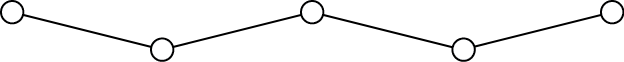
\includegraphics[width=.55\linewidth]{figures/5-path.png}} 
    \vspace{0.5cm}
    \caption{The path graph on 5 vertices. This is the smallest example of a graph that is not levelable.}
\end{figure}

\begin{example} \label{ex:5-path}
Let $P$ denote the path on 5 vertices $V(P) = \br{v_1, \dots, v_5}$, and edge set $E(G) = \br{\br{v_i, v_{i+1} \; | \; i = 1, \dots, 4}}$. Then 
\begin{equation*}
\begin{aligned}
F_1 &= \br{v_1, v_3, v_5}, \\
F_2 &= \br{v_2, v_4} \\
F_3 &= \br{v_1, v_4}, \textrm{ and } \\
F_4 &= \br{v_2, v_5}
\end{aligned}
\end{equation*}
are facets of $\ind(P)$. If $P$ were levelable, then there exists a valid simultaneous solution $(v_1, \dots, v_5)$ to $S(F_i) - S(F_i) = |F_i| - |F_{i+1}|$ for $i = 1, 2, 3$. For $i = 1$, we have
\begin{equation} \label{eq:5-path-1}
v_1 + v_3 + v_5 - v_2 - v_4 = 3 - 2 = 1.
\end{equation}
For $i = 2$, we have
\begin{equation*}
v_2 + v_4 - v_1 - v_4 = 2 - 2 = 0,
\end{equation*}
which gives $v_1 = v_2$. Then, for $i = 3$, we have
\begin{equation*}
v_1 + v_4 - v_2 - v_5 = 2 - 2 = 0.
\end{equation*}
Using the fact that $v_1 = v_2$ gives $v_4 = v_5$. If we apply these results to \eqref{eq:5-path-1}, we get that $v_3 = 1$, which gives a contradiction. So $P$ is not levelable.
\end{example}

We will in fact verify this result in \autoref{ch:non-levelable-results} as a consequence of \autoref{thm:graph-partitions}.

A natural question that follows is whether the path on 5 vertices acts as an obstruction to the levelable condition for a graph $G$ if it is an induced subgraph of $G$. However, a counterexample to this statement is given by the following:

\begin{example} \label{ex:5-path-induce} If $P$ is the path on 5 vertices $V(P) = \br{v_1, \dots, v_5}$ where $v_1$ and $v_5$ are the endpoints of the path, then the graph $G$ constructed by adding an additional vertex $v_6$ with edges $\br{v_2, v_6}$ and $\br{v_3, v_6}$ is a graph that has the path on 5 vertices as an induced subgraph (by removing $v_6$) and is levelable. 
\begin{figure}[bth]
    \myfloatalign
    \vspace{0.3cm}
    {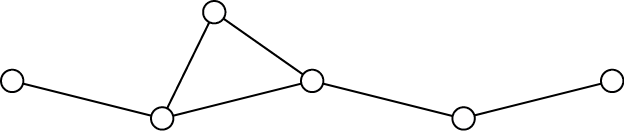
\includegraphics[width=.55\linewidth]{figures/5-path-induce.png}} 
    \vspace{0.2cm}
    \caption{The graph $G$ in \autoref{ex:5-path-induce}. The path on 5 vertices is an induced subgraph of $G$ by removing the highlighted vertex.}
\end{figure}
The facets of its independence complex are
\begin{equation*}
\begin{aligned}
&F_1 = \br{v_1, v_5, v_6}, \\
&F_2 = \br{v_1, v_3, v_5}, \\
&F_3 = \br{v_1, v_4, v_6}, \\
&F_4 = \br{v_2, v_5}, \\
&F_5 = \br{v_2, v_4}
\end{aligned}
\end{equation*}
and a valid solution to the corresponding levelable condition system is given by
$(v_1, v_2, v_3, v_4, v_5, v_6)= (2, 3, 2, 2, 2, 2)$.
\end{example}

While having the path on 5 vertices as an induced subgraph is not a strong enough condition to preclude levelability, we will later prove a result using the idea of an obstruction in \autoref{thm:adjoinment}.


\section{Other observations} 
We used the data from our search to identify families of graphs that are levelable. Below is a summary of some of these results.

\subsection{Cycles and Wheels} \label{subsec:cycles-wheels}
\begin{definition}
A graph $G$ on $n$ vertices is called a \textbf{cycle graph} if its vertices can be labelled  $v_1, \dots, v_n$ such that the edge set is $E(G) = \br{\br{v_i, v_{i+1}} \; | \; i=1, \dots, n-1} \cup \br{\br{v_1, v_n}}$. Then the \textbf{wheel graph} on $n+1$ vertices is the graph with vertex set $V(G) \cup \br{v_{n+1}}$ and edge set $E(G) \cup \br{\br{v_{n+1}, v_i} \; | \; i = 1, \dots, n}$. 
\end{definition}
\begin{figure}[bth]
    \myfloatalign
    \subfloat
    {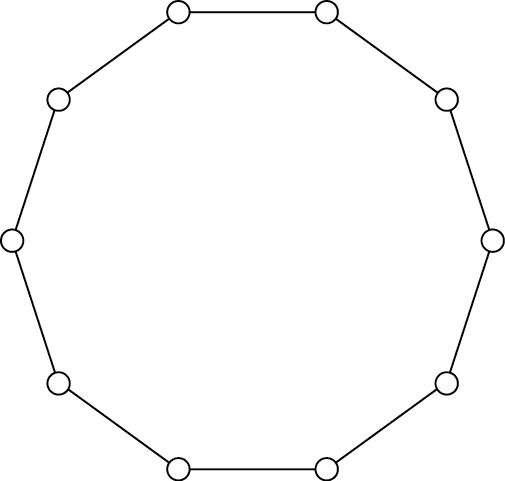
\includegraphics[width=.33\linewidth]{figures/cycle.png}} \qquad 
    \subfloat
    {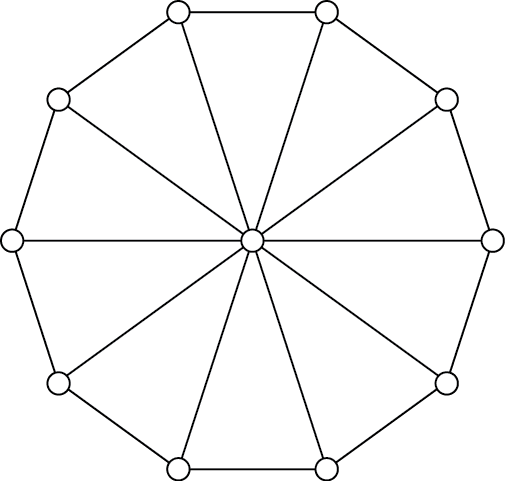
\includegraphics[width=.33\linewidth]{figures/wheel.png}} 
    \caption{The cycle graph on 10 vertices (left), and the wheel graph on 11 vertices (right)}
\end{figure}
Cycle graphs on 8 vertices or greater are not levelable, and the wheel graph on $n$ vertices is levelable if and only if the cycle on $n-1$ vertices is levelable. A general result for cycle graphs is given in \autoref{thm:cycles}. In \autoref{sec:adding-vertices-levelable} and \autoref{sec:adding-vertices-non-levelable} we show that adding a completely connected vertex to a graph does not change whether it is levelable.

\subsection{Long paths are not levelable} \label{subsec:paths} Paths on 5 vertices or greater are not levelable. This result has been generalized to \autoref{thm:graph-partitions}, which uses a proof based on this minimal example.

\subsection{Star graphs are levelable} \label{subsec:star}
\begin{definition} \label{def:star}
A graph $G$ on $n+1$ vertices is called a \textbf{star graph} if its vertices can be labelled $v_0, \dots, v_n$ such that the edge set is $E(G) = \br{\br{v_0, v_i} \; | \; i = 1, \dots, n}$. 
\end{definition}

\begin{figure}[bth]
    \myfloatalign
    {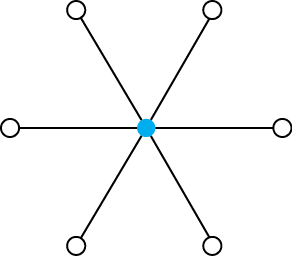
\includegraphics[width=.3\linewidth]{figures/star.png}} 
    \caption{The star graph on 7 vertices. The central vertex $v_0$ is shown in blue.}
\end{figure}

All star graphs are observed to be levelable. A generalization of this result is given in \autoref{thm:complete-multipartite}.

% Chapter 3
\chapter{Graphs that are levelable} % Chapter title

\label{ch:levelable-results} % For referencing the chapter elsewhere, use \autoref{ch:chaptername}

In this chapter we identify classes of graphs that are levelable. We also show that certain operations on graphs preserve levelability.

\section{Well-covered graphs}

The concept of a vertex cover was first introduced by \cite{Plummer1970}, is closely related to the maximal independent sets of a graph. Here we will connect the notions of minimal vertex covers to the facets of the independence complex, and use \autoref{thm:pure} to show that all well-covered graphs are levelable. Let us first define well-coveredness:

\begin{definition}
Let $G$ be a graph on $n$ vertices. A \textbf{vertex cover} of $G$ is a subset of vertices of $G$ such that every edge in $G$ is incident to some vertex in the vertex cover. A \textbf{minimal vertex cover} is a a vertex cover that fails to be a vertex cover if any of its vertices are removed. A graph $G$ is \textbf{well-covered} if every minimal vertex cover is of the same size. 
\end{definition}

We now relate the ideas of minimal vertex covers and maximal independent sets.

\begin{lemma}
A subset of vertices $X \subset V(G)$ is a minimal vertex cover if and only if $V(G) \setminus X$ is a maximal independent set. 
\end{lemma}
\begin{proof}
Let $G$ be a graph, and let $X \subset V(G)$ be a minimal vertex cover of $G$. Let $v, w \in V(G) \setminus X$. Then $\br{v, w} \not \in E(G)$, otherwise either $v$ or $w$ would be in $X$ in order for $X$ to be a vertex cover. So the complement of a vertex cover is an independent set. Furthermore, $V(G) \setminus X$ is maximal. If $(V(G) \setminus X)\cup\br{v'}$ (where $v' \in X$) was an independent set, then $(V(G) \setminus X) \cup {v'})^C = X \setminus \br{v'}$ would be a vertex cover. But then $X$ is not a minimal vertex cover. 
\end{proof}

Finally, we will apply \autoref{thm:pure} to show well-covered graphs are levelable.

\begin{theorem}
All well-covered graphs are levelable.
\end{theorem}
\begin{proof}
Let $G$ be a graph and $X_1, \dots, X_t$ denote the minimal vertex covers of $G$. Let  $F_i = V(G) \setminus X_i$ for $i = 1, \dots, t$. Then $F_1, \dots, F_t$ are maximal independent sets of $G$. If $G$ is well-covered, then $|X_1| =  \cdots = |X_t| = \lambda$. But then for any $i$, we have that $|F_i| = |V(G)| - |X_i| = |V(G)| - \lambda$. So $|F_1| = \cdots = |F_t| = |V(G)| - \lambda$. That is, all facets of the independence complex are the same size. Then, by \autoref{thm:pure}, $G$ is levelable.
\end{proof}

\section{Caterpillar graphs that are levelable} \label{sec:caterpillar}

We now discuss a particular type of graph called caterpillar graphs.

\begin{definition}
A graph $G$ is called a \textbf{caterpillar graph} if all the vertices of $G$ are all within distance 1 of a central path, and $G$ is cycle-free. Vertices that are not on the central path are called \textbf{legs} of $G$.
\end{definition}
\begin{figure}[bth]
    \myfloatalign
    {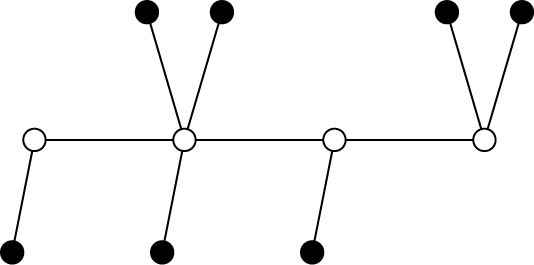
\includegraphics[width=.42\linewidth]{figures/caterpillar.png}} 
    \caption{An example of a caterpillar graph. Vertices on the central path are shown in white, and legs are shown in black.}
\end{figure}

In general, it is not true that all caterpillar graphs are levelable. As a counterexample, a caterpillar with no legs and a central path of length 5 is simply the path on 5 vertices, which is not levelable. However, the following theorem gives us a sufficient condition for levelability on caterpillar graphs.

\begin{theorem} \label{thm:caterpillar}
Let $G$ be a caterpillar graph. If every vertex on the central path of $G$ has at least one leg (except perhaps the endpoints of the path), then $G$ is levelable.
\end{theorem}

\begin{proof}
Suppose $G$ is caterpillar graph on $N$ vertices. Denote vertices on the central path by $p_1, \dots, p_n$. Let $L_i$ denote the set of legs that are adjacent to $p_i$. We can assume, without loss of generality, that $L_i \neq \emptyset$ for all $i$. If any of the endpoints $p_1$ or $p_n$ does not have a leg, then we can relabel the vertices such that $p_1$ as a leg of $p_2$ and/or $p_{n}$ as a leg of $p_{n-1}$. Let us then set a solution to the system in \autoref{thm:level-condition} as follows:
\begin{enumerate}
\item for any leg vertex $v_\alpha \in L_1 \cup \dots \cup L_n$, set $v_\alpha = 2$, and
\item for a vertex $p_i$ on the central path, set $p_i =  |L_i| + 1 $.
\end{enumerate}
Note that each $L_i$ is an independent set, since every leg in $L_i$ is adjacent to $p_i$, and if two legs in $L_i$ were adjacent this would create a cycle. Then, if $\ang{F_1, \dots, F_t}$ denotes the maximal independent sets of $G$, then each $F$ must satisfy either $p_i \in F$ or $L_i \subset F$ for each $i = 1, \dots, n$. Consider any two facets $F_a$ and $F_b$. Let $X = \br{i \; | \; i = 1, \dots, n}$, $A = \br{i \; | \; L_i \in F_a}$, and $B = \br{i \; | \; L_i \in F_b}$. The equation
\begin{equation*}
\begin{aligned}
S(F_a) - S(F_b) = |F_a| - |F_b|.
\end{aligned}
\end{equation*}
can therefore be written 
\begin{equation*}
\begin{aligned}
\left[S\left( \bigcup_{i \in A} L_i \right) + 
S\left( \bigcup_{i \in X \setminus A} \br{p_i} \right) \right] - 
\left[S\left( \bigcup_{i \in B} L_i \right) +
S\left( \bigcup_{i \in X \setminus B} \br{p_i} \right) \right] \\= \left|\bigcup_{i \in A} L_i \right| + |X \setminus A| - \left|\bigcup_{i \in B} L_i \right| -|X \setminus B|.
\end{aligned}
\end{equation*}
Substituting our proposed solution yields
\begin{equation*}
\begin{aligned}
2 \sum_{i \in A} |L_i| + \sum_{i \in X\setminus A} (|L_i| + 1)  - 2 \sum_{i \in B} |L_i| - \sum_{i \in X \setminus B} (|L_i| + 1) \\
= \sum_{i \in A} |L_i| + |X \setminus A| - \sum_{i \in B} |L_i| - |X \setminus B|,
\end{aligned}
\end{equation*}
which, by cancelling sums on each side, can be simplified to 
\begin{equation*}
\begin{aligned}
 \sum_{i \in A} |L_i|  +  \sum_{i \in X\setminus A} (|L_i| + 1) - \sum_{i \in B} |L_i| -  \sum_{i \in X \setminus B} (|L_i| + 1) 
= |X \setminus A| - |X \setminus B|.
\end{aligned}
\end{equation*}
Expanding constants in the sums yields
\begin{equation*}
\begin{aligned}
 \sum_{i \in A} |L_i|  +  \sum_{i \in X\setminus A} |L_i|  + |X \setminus A| - \sum_{i \in B} |L_i| -  \sum_{i \in X \setminus B} |L_i| - |X \setminus B|
= |X \setminus A| - |X \setminus B|,
\end{aligned}
\end{equation*}
i.e.,
\begin{equation*}
\begin{aligned}
 \sum_{i \in A} |L_i|  +  \sum_{i \in X\setminus A} |L_i|  - \sum_{i \in B} |L_i| -  \sum_{i \in X \setminus B} |L_i| = 0,
\end{aligned}
\end{equation*}
or equivalently
\begin{equation*}
\begin{aligned}
 \smashoperator{ \sum_{i \in A \cup (X \setminus A)}} |L_i|  \; \; - \; \; \smashoperator{\sum_{i \in B \cup (X \setminus B)}} |L_i|= 0,
\end{aligned}
\end{equation*}
since any set and its complement are disjoint. Since $F_1, \dots, F_t$ are all the facets of $G$, we have found a solution that satisfies $S(F_k) - S(F_{k+1}) = |F_k| - |F_{k+1}|$ for all $i$, and by \autoref{thm:level-condition} $G$ is levelable.
\end{proof}

\begin{example} \label{ex:levelable-caterpillar}(Levelable Caterpillar Graph) 
Let $G$ be a graph with:
\begin{itemize}
\item vertex set $V(G) = \br{p_1, p_2, p_3, q_1, \dots, q_6}$, and 
\item edge set $E(G) = \br{
\br{p_1, p_2},
\br{p_2, p_3},
\br{p_1, q_i \, | \, i = 1, 2},
\br{p_2, q_3},
\br{p_3, q_i \, | \, i = 4, 5, 6}
}.$
\end{itemize}
For a picture, see \autoref{fig:caterpillar-ex}. 

Here $p_1, p_2, p_3$ form the central path, and their corresponding leg vertices are $L_1 = \br{q_1, q_2}$, $L_2 = \br{q_3}$, and $L_3 = \br{q_4, q_5, q_6}$. As per \autoref{thm:caterpillar}, we will show that we can construct a levelable solution by setting
\begin{itemize}
\item $q_1 = \cdots = q_6 = 2$, 
\item $p_1 = |L_1| + 1 = 3$,
\item $p_2 = |L_2| + 1 = 2$, and
\item $p_3 = |L_3| + 1 = 4$.
\end{itemize}
Now, the maximal independent sets of $G$ are
\begin{itemize}
\item $F_1 = \br{p_1} \cup L_2 \cup \br{p_3} = \br{p_1, p_3, q_2}$,
\item $F_2 = \br{p_1} \cup L_2 \cup L_3 = \br{p_1, q_3, q_4, q_5, q_6}$,
\item $F_3 = L_1 \cup \br{p_2} \cup L_3 = \br{p_2, q_1, q_2, q_4, q_5, q_6}$,
\item $F_4 = L_1 \cup L_2 \cup \br{p_3} = \br{q_1, q_2, q_3, p_3}$
\item $F_5 = L_1 \cup L_2 \cup L_3 = \br{q_1, q_2, q_3, q_4, q_5, q_6}$,
\end{itemize}
We therefore have 4 equations in our system. The first is given by $S(F_1) - S(F_2) = |F_1| - |F_2|$, where 
\begin{itemize}
\item $S(F_1) = S(\br{p_1, p_3}) + S(L_1) = (3 + 4) + (2) = 9$,
\item $S(F_2) = S(\br{p_1}) + S(L_2 \cup L_3) =  (3) + (4 \cdot 2) = 11$,
\item $|F_1| = 3$, and
\item $|F_2| = 5$. 
\end{itemize} 
Then the first equation is satisfied, since
$$
S(F_1) - S(F_2) = 9 - 11 = -2 = 3 - 5 = |F_1| - |F_2|.
$$
The second equation is given by $S(F_2) - S(F_3) = |F_2| - |F_3|$, where
\begin{itemize}
\item $S(F_3) = S(\br{p_2}) + S(L_1 \cup L_3) = (2) + (5 \cdot 2) = 12$, and
\item $|F_3| = 6$.
\end{itemize} 
The second equation is satisfied since
$$
S(F_2) - S(F_3) = 11 - 12 = -1 = 5 - 6 = |F_2| - |F_3|.
$$
The third equation is given by $S(F_3) - S(F_4) = |F_3| - |F_4|$ where
\begin{itemize}
\item $S(F_3) = S(L_1 \cup L_2) + S(\br{p_3}) = (3 \cdot 2) + (3+1) = 10$, and
\item $|F_4| = 4$.
The third equation is satisfied, since
$$
S(F_3) - S(F_4) = 12 - 10 = 2 = 6 - 4 = |F_3| - |F_4|.
$$
\end{itemize}
The fourth and final equation is given by $S(F_4) - S(F_5) = |F_4| - |F_5|$ where
\begin{itemize}
\item $S(F_5) = S(L_1 \cup L_2 \cup L_3) = (6 \cdot 2) = 12$ and
\item $|F_5| = 6$.
\end{itemize}
This equation is also satisfied since 
$$
S(F_4) - S(F_5) = 10 - 12 = -2 = 4 - 6 = |F_4| - |F_5|,
$$
and so we have found a valid solution and $G$ is therefore levelable.
\end{example}
\begin{figure}[bth] 
    \myfloatalign
    \vspace{0.25cm}
    {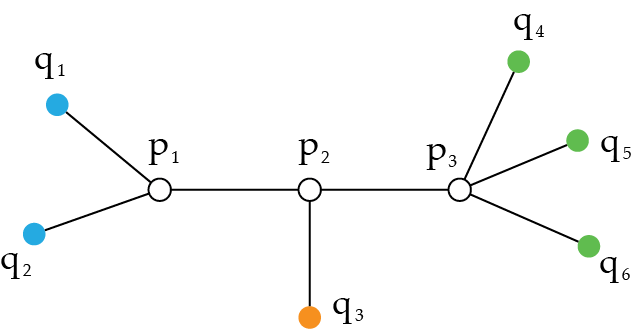
\includegraphics[width=.45\linewidth]{figures/caterpillar-ex.png}} 
    \caption{The levelable caterpillar graph described in \autoref{ex:levelable-caterpillar}. The central path is shown in white, while $L_1$, $L_2$, and $L_3$ are shown in blue, orange, and green respectively.} \label{fig:caterpillar-ex}
\end{figure}

It is interesting to note that every caterpillar graph on 4 or fewer vertices must satisfy the condition in \autoref{thm:caterpillar}. For example, the path graph on 4 vertices can be thought of as a caterpillar on a central path of 2 vertices, each adjacent to one leg vertex. However, any path graph on $n \geq 5$ vertices does not satisfy the condition, and none of these are levelable. This observation leads us to the converse statement of \autoref{thm:caterpillar}:

\begin{question}
Let $G$ be a caterpillar graph on 5 or greater vertices. If $G$ is levelable, does every vertex on the central path has at least one leg?
\end{question}

We also observe that this hypothesis is consistent with our computer search. That is, all levelable caterpillars on $n \leq 10$ vertices satisfy the condition in \autoref{thm:caterpillar}, and every non-levelable caterpillar has at least one vertex on the central path that does not have a leg.

\section{Complete multipartite graphs}

In this section we show that all complete multipartite graphs are levelable using a result from \cite{VanTuyl2010}. First, let us state the result.

\begin{theorem}[Theorem 12(iii) from \cite{VanTuyl2010}] \label{thm:pairwise-disjoint}
Any simplicial complex $\Delta$ with pairwise disjoint facets is levelable.
\end{theorem}

This result can be related to independence complexes on complete multipartite graphs, which are defined as follows:

\begin{definition} \label{def:complete-multipartite}
Let $G$ be graph on $n_1 + \dots + n_k$ vertices. Then $G$ is a \textbf{complete multipartite} graph or more specifically, a \textbf{complete $k$-partite graph} if its vertex set $V(G)$ can be expressed as $k$ disjoint sets $V_1$, \dots, $V_k$ such that the edge set $E(G)$ can be written 
$$
E(G) = \br{ \br{v, w} \, | \, v \in V_i, \, w \in V_j, \, i \neq j }.
$$
\end{definition}

\begin{theorem} \label{thm:complete-multipartite}
All complete multipartite graphs are levelable.
\end{theorem}

\begin{proof} 
If $G$ is a complete multipartite graph, then its maximal independent sets are pairwise disjoint. We will prove this by showing that the $k$ maximal independent sets of $G$ are exactly the $k$ disjoint sets $V_1, \dots, V_k$ as described in \autoref{def:complete-multipartite}. Notice first that the edge set does not contain any edges with endpoints within the same $V_i$. Thus each $V_i$ is an independent set. Then, notice that every vertex $v \in V_i$ is adjacent to all vertices $w \in V(G) \setminus V_i$. Thus $V_i$ is a maximal independent set. By construction $V_1, \dots, V_k$ are pairwise disjoint. Therefore by \autoref{thm:pairwise-disjoint}, all complete multipartite graphs are levelable.
\end{proof}

We can apply this result to star graphs, which were observed to be levelable in \autoref{subsec:star}.

\begin{corollary}
All star graphs are levelable.
\end{corollary}

\begin{proof}
The star graph on $n+1$ vertices is a complete 2-partite (``bipartite") graph. If we label the vertices as in \autoref{def:star}, then $V_1 = \br{v_0}$  and $V_2 = \br{v_1, \dots, v_{n}}$ give two disjoint vertex subsets such that 

\begin{enumerate}
\item there are no edges between pairs of vertices where both vertices are from either $V_1$ and $V_2$, and
\item all vertices in $V_1$ are adjacent to all vertices in $V_2$, since $v_0$ is adjacent to the other $n$ vertices.
\end{enumerate}

Thus, the star graph is a complete bipartite, and levelable by \autoref{thm:complete-multipartite}.
\end{proof}

\begin{figure}[bth]
    \myfloatalign
    {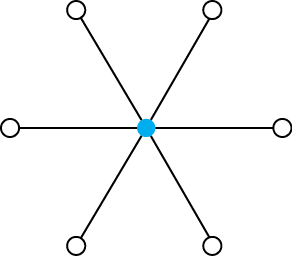
\includegraphics[width=.3\linewidth]{figures/star.png}} 
    \caption{The star on 7 vertices. The central vertex $v_0$ is shown in blue.}
\end{figure}



% --------------------------------------------------------------------------
% -------------------------------------------------------------------------

\section{Graph expansions}
We will now discuss operations on graphs that preserve the levelable property. Given a graph that is levelable, we can construct other levelable graphs by applying an "expansion" operation on the graph.

\begin{definition} \label{def:graph-expansion}
Let $G$ be a graph on $n$ vertices. A \textbf{graph expansion} $G'$ of $G$ is any graph where each vertex $v_i$ is replaced with a set of independent vertices $V_i = \br{v_{i, 1}, \cdots, v_{i, k_i}}$, and a vertex $v \in V_i$ is adjacent to a vertex in $w \in V_j$ if and only if $v_i$ and $v_j$ are adjacent in $G$. The sets $V_1, \dots, V_n$ that make up $V(G')$ are called \textbf{replica sets}, and a vertex $v \in V_i$ is called a \textbf{replica} of the \textbf{original vertex} $v_i$. Furthermore, we call $G'$ a \textbf{$k$-uniform expansion} if $|V_i| = k$ for $k = 1, \dots, n$. 
\end{definition}

An illustration of a graph expansion is given in \autoref{fig:expansion-ex}.

\begin{figure}[bth] 
    \myfloatalign
    \subfloat
    {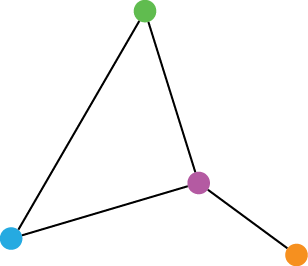
\includegraphics[width=.25\linewidth]{figures/expansion-before.png}} \\
    \subfloat
    {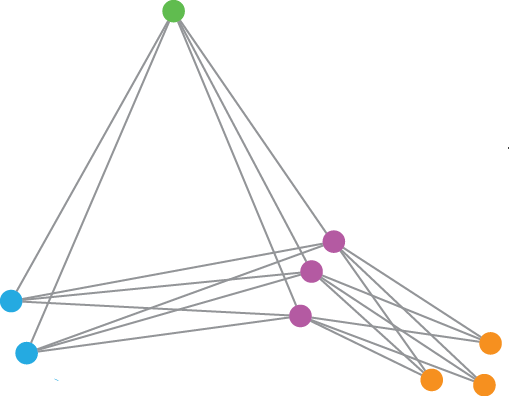
\includegraphics[width=.40\linewidth]{figures/expansion-nonuniform.png}} \\
    \subfloat
    {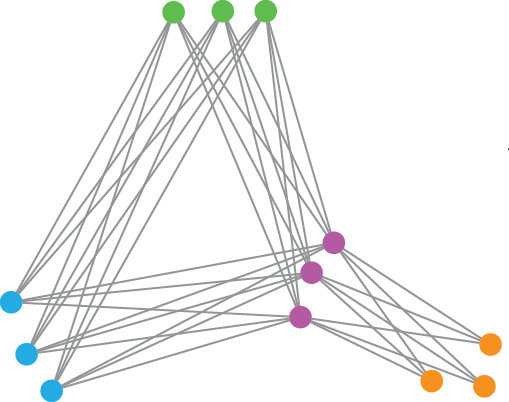
\includegraphics[width=.47\linewidth]{figures/expansion-uniform.png}} 
    \caption{A graph $G$ on 4 vertices (top); a non-uniform expansion of $G$ (middle); a 3-uniform expansion of $G$ (bottom). Replica sets are shown in the same colour as their original vertex.}\label{fig:expansion-ex}
\end{figure}

\begin{theorem} \label{thm:expansion}
Let $G$ be a levelable graph. Then any uniform expansion $G'$ of $G$ is levelable.
\end{theorem}
\begin{proof}
Since $G$ is levelable, let $(x_1, \dots, x_n)$ be a solution to \autoref{thm:level-condition}. Let $G'$ be a $k$-uniform expansion of $G$, and label the vertices $w_1, \dots, w_{nk}$ such that the first $k$ vertices correspond to $V_1$ in the expansion, the next $k$ vertices correspond to $V_2$, and so on. Then we claim that the $nk$-tuple $$(x_{1,1}, \dots, x_{1, k}, x_{2, 1}, \dots, x_{2, k}, \dots,x_{n, 1}, \dots, x_{n, k})$$ where $x_{i, j} = x_i$ is a solution to the the system in \autoref{thm:level-condition} for $G'$. 
First, we will show that the maximal independent sets of $G'$ are of the form 
\begin{equation*} \label{eq:expansion-union}
F' = \bigcup_{\br{\alpha: \, v_\alpha \in F}}  V_\alpha 
\end{equation*}
where $F$ is a maximal independent set in $G$. First, we note that for any maximal independent set $F'$ of $G'$, if some replica vertex is in $F'$, then all other vertices in its replica set will also be in $F'$. So $F'$ must be a union of replica sets.

It then follows from the construction of the expansion that replica sets are adjacent if and only if their corresponding original vertex was adjacent. That is,
$$
V_i \cup V_j \, \textrm{is an independent set} \Leftrightarrow N(V_i) \cap V_j = \emptyset \Leftrightarrow \br{v_i, v_j} \not \in E(G).
$$
We can then conclude that the maximal independent sets of $G'$ arise precisely out of corresponding maximal independent sets of $G$. 

Now, if $F_1, \dots, F_t$ are the maximal independent sets of $G$, then $F_1' \dots, F_t'$ are the maximal independent sets of $G'$. Consider any of the $t-1$ equations in \autoref{thm:level-condition}, each of the form
\begin{equation*}
\begin{aligned}
S(F_i') - S(F_{i+1}') = |F_i'| - |F_{i+1}'|.
\end{aligned}
\end{equation*}
Note that each facet $F'$ has $k$ times as many vertices as $F$, and so $|F'| = k |F|$. In addition, by substituting our proposed solution, for any replica set $V_i$, $S(V_i) = k v_i$. Since each $F'$ is made of a union of replica sets and replica sets are pairwise disjoint, $S(F') = k S(F)$. Therefore, we can write the above equation as
\begin{equation*}
\begin{aligned}
kS(F_i) - kS(F_{i+1}) = k|F_i| - k|F_{i+1}|,
\end{aligned}
\end{equation*}
to which there is a solution when $G$ is levelable.
\end{proof}

\section{Adding vertices} \label{sec:adding-vertices-levelable}

Here we will show that adding vertices (up to a certain number) adjacent to all existing vertices of the graph preserves the levelable condition.

\begin{theorem} \label{thm:vertex-add}
Let $G$ be a levelable graph and let $F_1, \dots, F_t$ denote the facets of $\ind(G)$. Define $G'$ to be the graph with vertex set $V(G') = V(G) \cup \br{w_1, \dots, w_m}$ and edge set $E(G') = E(G) \cup \br{\br{v_i, w_j} \; | \; v_i \in V(G), j = 1, \dots, m}$, where $m \leq |F_t|$. Then $G'$ is levelable.
\end{theorem}

\begin{proof}
If $F_1, \dots, F_t$ are the facets of $\ind(G)$, Then $F_1, \dots, F_t, \br{w_1, \dots, w_m}$ are the facets of $\ind(G')$, since each $w_i$ is adjacent to every vertex in $V(G)$ but independent of all $w_j$ for $i \neq j$. Since $G$ is levelable, there exists some solution $(a_1, \dots, a_n)$ to the system in \autoref{thm:level-condition} for $G$.

If we set $b_1 = \cdots b_{m-1} = 2$ and $b_m = S(F_t) - m + 2 - |F_t|$, then $(a_1, \dots, a_n, \allowbreak b_1, \dots, b_m)$ is a solution to the system of $t$ equations for $G'$, where $b_i$ corresponds to $w_i$. 

Notice first that the first $t-1$ equations $S(F_i) - S(F_{i+1})  = |F_i| - |F_{i+1}|$ for $t = 1, \dots, t-1$ are unchanged from $G$, and are independent of $w_1, \dots, w_m$. Then, the $t^{\textrm{th}}$ equation is 
$$
S(F_t) - b_1 - \cdots - b_m = |F_t| - m.
$$
If we take $b_1 = \cdots = b_{m-1} = 2$ and $b_m = S(F_t) - m + 2 - |F_t| \geq 2$, then
\begin{equation*}
\begin{aligned}
S(F_t) - b_1 - \cdots - b_m &= S(F_t) - 2(m-1) - S(F_t) + m - 2 + |F_t| \\ &= -2m + 2  + m  - 2 +| F_t| \\&= -m + |F_t|.
\end{aligned}
\end{equation*}
as required. Furthermore $b_m \geq 2$, since, when $|F_t| \geq m$ we have
$$
b_m = S(F_t) - m + 2 - |F_t| \geq S(F_t) - |F_t| + 2 - |F_t| \geq 2|F_t| - |F_t| + 2 - |F_t| = 2.
$$
Thus a valid solution exists and $G'$ is levelable.
\end{proof}

\begin{example} \label{ex:star-add}
Let $G$ be the star on 4 vertices labelled $v_1, \dots, v_4$ where $v_1$ is the central vertex. Since $G$ is a graph on only 4 vertices, by \autoref{thm:small} it is levelable. The two maximal independent sets of $G$ are given by 
$F_1 = \br{v_1}$ and 
$F_2 = \br{v_2, v_3, v_4}$.
Now, let $G'$ be the graph with vertex set $V(G') = V(G) \cup \br{w_1, w_2}$ and edge set $E(G) = \br{ \br{v_i, w_j} \; | \; i = 1, \dots, 4; \, j = 1, \dots, 2}$. Since $G$ is levelable, there exists a solution to the system in \autoref{thm:level-condition}. In particular, a solution is given by $(v_1, v_2, v_3, v_4) = (4, 2, 2, 2)$:
$$
S(F_1) - S(F_2) = 4 - 3(2) = -2 = 1 - 3 = |F_1| - |F_2|.
$$
The corresponding system for $G'$ has one additional facet $F_3 = \br{w_1, w_2}$ and a solution given by $(v_1, v_2, v_3, v_4, w_1, w_2) = (4, 2, 2, 2, 2, 3)$, where the value of $w_3$ arises from $S(F_2) - m + 2 - |F_2| = 6 - 2 + 2 - 3 = 3$ as per \autoref{thm:vertex-add}. Indeed, this is a solution since
$$
S(F_2) - S(F_3) = 3(2) - 2 - 3 = 1 = 3 - 2 = |F_2| - |F_3|,
$$
and $G$ is levelable.

\begin{figure}[h]
    \myfloatalign
    \subfloat
    {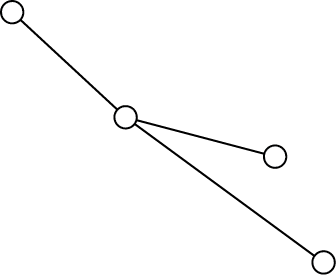
\includegraphics[width=.26\linewidth]{figures/4-star-before.png}} \qquad
    \subfloat
    {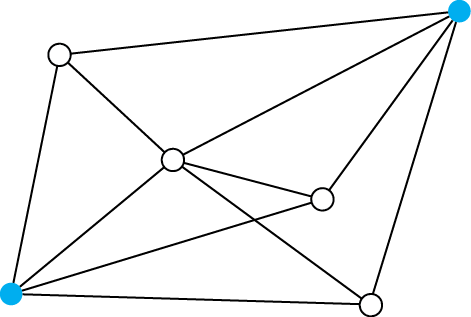
\includegraphics[width=.37\linewidth]{figures/4-star-addition.png}}
    \caption{The star on 4 vertices (left) and the graph $G'$ (right) constructed in \autoref{ex:star-add} by adding two additional vertices shown in blue.}
\end{figure}

\end{example}


\chapter{Graphs that are not levelable}

\label{ch:non-levelable-results}

In this chapter we discuss conditions that preclude levelability. In particular, in \autoref{sec:large-cycles} we show that large cycles are not levelable, and in \autoref{sec:criteria} we introduce a criterion on the independent sets of a graph that allows us to conclude that certain trees, including all paths on large numbers of vertices, are not levelable. Finally, in \autoref{sec:adjoinment} we show that attaching a non-levelable graph in a certain way will always result in a non-levelable graph.

\section{Large cycles} \label{sec:large-cycles}

In \autoref{subsec:cycles-wheels}, we noted that cycles were observed to fail to be levelable. We begin this chapter by proving this fact for cycles of arbitrary size $n \geq 8.$

\begin{theorem}\label{thm:cycles}
Let $G$ be the cycle graph on $n$ vertices, where $n \geq 8$. Then $G$ is not levelable.
\end{theorem}
\begin{proof}
Label the $n$ vertices clockwise in increasing order $v_1, \dots, v_n$. Then we have that the edge set is $E(G)= \br{ \br{v_i, v_{i+1}} \, | \,i = 1, \dots, n-1} \cup \br{\br{v_1, v_n}}$. Suppose, for a contradiction that $(x_1, \dots, x_n)$ is a solution that satisfies \autoref{thm:level-condition}.

First, we note that a maximal independent set $F$ of $G$ is a selection of vertices from the cycle such that any vertex in $F$ is distance 2 or  3 from another vertex in $F$ , but not more. These are independent sets, since we have chosen vertices that are not adjacent in the cycle. Furthermore, these are maximal since any smaller selection would have a gap of 3 or more vertices in the cycle. We could then properly include such a selection in a larger independent set by taking a middle vertex in the gap of 3 or more vertices. 

\noindent
\underline{Case}: $n$ is even.  
Take $F_1$ to be the set of even-numbered vertices $F_1 = \br{v_2, v_4, \dots, v_n}$, and take $F_2$ to be the set of all even numbered vertices up to $v_{n-4}$ inclusive, and $v_{n-1}$. So $F_2 = \br{v_2, v_4, \dots, v_{n-4}, v_{n-1}}$. Then  $S(F_1) - S(F_2) = |F_1| - |F_2|$, i.e.,
\begin{equation*}
\begin{aligned}
(x_2 + x_4 + \cdots + x_n) - (x_2, x_4, \dots, x_{n-4}, x_{n-1}) &= \frac{n}{2} - \left(\frac{n}{2} - 1\right) = 1,
\end{aligned}
\end{equation*}
which reduces to
\begin{equation}\label{eq:cycle-1}
\begin{aligned}
x_{n-2} + x_n - x_{n-1} &= 1.
\end{aligned}
\end{equation}
Take $F_3 = \br{v_2, v_4, \dots, v_{n-6}, v_{n-3}, v_{n-1}}$ and $F_4 = \br{v_2, v_4, \dots, v_{n-6}, v_{n-3}, v_n}$. Then $S(F_3) - S(F_4) = |F_3| - |F_4|$, i.e.,
\begin{equation*}
\begin{aligned}
(x_2, x_4, \dots, x_{n-6}, x_{n-3}, x_{n-1}) - (x_2, x_4, \dots, x_{n-6}, x_{n-3}, x_{n-1}) = 0
\end{aligned}
\end{equation*}
which reduces to
\begin{equation} \label{eq:cycle-2}
\begin{aligned}
x_{n-1} & = x_n.
\end{aligned}
\end{equation}
Combining the information from \eqref{eq:cycle-1} and \eqref{eq:cycle-2} we obtain $x_{n-2} + x_n - x_{n-1} = x_{n-2} + x_n - x_n = 1$ which gives a contradiction, since we require all $x_i \geq 2$. Thus $G$ is not levelable for even $n$.

\noindent
\underline{Case}: $n$ is odd. 
Take $F_1$ to be the even-labelled vertices $\br{v_2, \dots, v_{n-1}}$ and $F_2 = \br{v_1, v_3, v_6, v_8 \dots, v_{n-1}}$. Then $S(F_1) -S(F_2) = |F_1| - |F_2| = 0$, i.e.,
\begin{equation*}
\begin{aligned}
(x_2 + \dots + x_{n-1}) - (x_1 + x_3 + x_6 + x_8 + x_{n-1}) &= 0 
\end{aligned}
\end{equation*}
which reduces to
\begin{equation}\label{eq:odd1}
\begin{aligned} 
x_2 + x_4 &= x_1 + x_3.
\end{aligned}
\end{equation}
Then take $F_3 = \br{v_1, v_4, v_6, v_8 \dots, v_{n-1}}$, and $S(F_2) -S(F_3) = |F_2| - |F_3|$ gives
$$
(x_1 + x_3 + x_6 + x_8 + \cdots + x_{n-1}) - (x_1 + x_4 + x_6 + x_8 + \cdots + x_{n-1}) = 0
$$
which reduces to
\begin{equation}
\begin{aligned}
\label{eq:odd2}
x_3 &= x_4.
\end{aligned}
\end{equation}
Combining the result from \eqref{eq:odd1} and \eqref{eq:odd2} gives $x_1 = x_2$. Now, take $F_4 = \br{v_2, v_4, v_6, \allowbreak \dots,  v_{n-5}, v_{n-2}, v_n}$. Since $S(F_3) -S(F_4) = |F_3| - |F_4| = 0$, we have that
\begin{equation*}
\begin{aligned}
(x_1 + x_4 + x_6 + x_8 + \cdots + &x_{n-3} + x_{n-1}) \\ &- (x_2 + x_4 + x_6 + \cdots+ x_{n-5} + x_{n-2}+ x_n) = 0, 
\end{aligned}
\end{equation*}
i.e.,
\begin{equation}
\begin{aligned}\label{odd3}
x_{n-3} + x_{n-1} &= x_{n-2} + x_n.
\end{aligned}
\end{equation}
Then take $F_5 =\br{ v_2, v_4, v_6, \dots, v_{n-5}, v_{n-3}, v_n}$. Since $S(F_4) -S(F_5) = |F_4| - |F_5| = 0$,
\begin{equation*}
\begin{aligned}
(x_2+ x_4+ x_6 + \cdots + x_{n-5} + &x_{n-2}+ x_n)  \\ &- (x_2+ x_4+ x_6 + \cdots + x_{n-5} + x_{n-3}+ x_n) = 0, 
\end{aligned}
\end{equation*}
which reduces to
\begin{equation} \label{odd4}
x_{n-2} = x_{n-3}.
\end{equation}
Combining the equalities from \eqref{odd3} and \eqref{odd4} yields $x_{n-1} = x_n$. Now, take $F_6 = \br{v_1, v_4, v_6, \dots, v_{n-5}, v_{n-2}}$. Then $S(F_5) - S(F_6) = |F_5| - |F_6|$ gives
\begin{equation*}
\begin{aligned}
\label{odd5}
(x_2+ x_4+ x_6 + \cdots + x_{n-5} + &x_{n-3}+ x_n) \\ &- (x_1 + x_4 + x_6 + \cdots + x_{n-5} + x_{n-2}) = 1,
\end{aligned}
\end{equation*}
and cancelling the common terms yields
\begin{equation*}
\begin{aligned}
(x_2+  x_{n-3}+ x_n) - (x_1 + x_{n-2}) &= 1. \\
\end{aligned}
\end{equation*}
But since $x_{n-3} = x_{n-2}$ and $x_2 = x_1$, we have that $x_n = 1$, which again, gives a contradiction since we require that any $x_i \geq 2$. So $G$ is also not levelable if $n$ is odd.
\end{proof}

\section{Criteria on vertex partitions} \label{sec:criteria}

In \autoref{sec:smallest}, we showed that the path on 5 vertices is not levelable. Here, we give a generalization of that result using a similar proof. Using this result, we rule out certain classes of tree graphs in \autoref{cor:balanced-trees}, which also lets us conclude that long paths are not levelable in \autoref{cor:long-paths}.

\begin{theorem} \label{thm:graph-partitions}
Let $G$ be a graph on $n$ vertices. If the vertex set of $G$, $V(G)$ has a partition $V(G) = V_1 \cup  \cdots \cup  V_5 \cup W$, and $Y \subset W$ such that 
\begin{equation} \label{eq:graph-partitions}
\begin{aligned}
F_1 &= V_1 \cup V_3 \cup V_5 \cup Y,\\
F_2 &= V_2 \cup V_4 \cup Y,\\
F_3 &= V_2 \cup V_5 \cup Y, \textrm{ and }\\
F_4 &= V_1 \cup V_4 \cup Y
\end{aligned}
\end{equation}
are maximal independent sets of $G$, then $G$ is not levelable.
\end{theorem}
\begin{proof}
Assume that $G$ is levelable. Then there exists some valid solution to the system in \autoref{thm:level-condition}. The first equation is given by
\begin{equation*}
\begin{aligned}
S(F_1) - S(F_2) = |F_1| - |F_2|.
\end{aligned}
\end{equation*}
Since $V_i$ and $V_j$ are disjoint for any $i \neq j$, this equation can be written as
\begin{equation*}
\begin{aligned}
S(V_1) + S(V_3) + S(V_5) + S(Y) - S(V_2) - S(V_4) - S(Y) \\
= |V_1| + |V_3| + |V_5| + |Y| - |V_2| - |V_4| -|Y|.
\end{aligned}
\end{equation*}
i.e., 
\begin{equation} \label{eq:5part1}
\begin{aligned}
S(V_1) + S(V_3) + S(V_5) - S(V_2) - S(V_4) = |V_1| + |V_3| + |V_5| - |V_2| - |V_4|.
\end{aligned}
\end{equation}
The second equation $S(F_2) - S(F_3) = |F_2| - |F_3|$ can similarly be written as
$$
S(V_2) + S(V_4)  +  S(Y) - S(V_1) - S(V_4) - S(Y) = |V_2| + |V_4| +|Y| - |V_1| - |V_4| - |Y|.
$$
Cancelling terms yields
\begin{equation} \label{eq:5part2}
\begin{aligned}
S(V_2) - S(V_1) = |V_2| - |V_1| .
\end{aligned}
\end{equation}
The final equation $S(F_3) - S(F_4) = |F_3| - |F_4|$ can be written as
\begin{equation*} 
\begin{aligned}
S(V_1) + S(V_4) + S(Y)- S(V_2) - S(V_5) - S(Y)= |V_1| + |V_4| + |Y|- |V_2| - |V_5| - |Y|,
\end{aligned}
\end{equation*}
that is,
\begin{equation} \label{eq:5part3}
\begin{aligned}
S(V_1) + S(V_4) - S(V_2) - S(V_5) = |V_1| + |V_4| -|V_2| - |V_5|.
\end{aligned}
\end{equation}
Applying the result from equation \eqref{eq:5part2} to \eqref{eq:5part3}, we obtain that
$$
S(V_1) + S(V_4) - S(V_2) - S(V_5) =  |V_4| - |V_5|  + S(V_1)  - S(V_2),
$$
i.e.,
\begin{equation} \label{eq:5part4}
\begin{aligned}
S(V_4) - S(V_5) &=  |V_4| - |V_5|.
\end{aligned}
\end{equation}
If we substitute the result from \eqref{eq:5part2} in the right-hand side of \eqref{eq:5part1}, we obtain
\begin{equation*}
\begin{aligned}
S(V_1) + S(V_3) + S(V_5) - S(V_2) - S(V_4) = S(V_1) + |V_3| + |V_5| - S(V_2) - |V_4|
\end{aligned}
\end{equation*}
Futhermore, applying the result from \eqref{eq:5part4} to the right-hand side of the above equation yields
$$
S(V_1) + S(V_3) + S(V_5) - S(V_2) - S(V_4) = S(V_1) + |V_3| + S(V_5) - S(V_2) + S(V_4).
$$
Cancelling common terms from both sides yields
$$
S(V_3) = |V_3|,
$$
but this means $G$ cannot be levelable. If a solution $(a_1, \dots, a_n)$ has $a_i \geq 2$ for all $i$, then it must be that $S(V_3) \geq 2 |V_3|$. 
\end{proof}
\noindent
We can apply the above result to trees to show that certain trees are not levelable. 

\begin{definition}
A graph $G$ is a \textbf{tree} if any two vertices $x$ and $y$ in $G$ can be connected by a unique simple path. That is, there is exactly one set of edges $\br{\br{x, v_1}, \dots, \br{v_n, y}}$ that connect $x$ and $y$. Furthermore, a \textbf{rooted tree} is a graph where one vertex has been designated the vertex. The \textbf{depth} of a vertex in a rooted tree is the length of the path from the vertex to the root. A vertex on a tree is called a \textbf{leaf} if it is connected only adjacent to one other vertex. The maximum depth of a leaf (or equivalently, the length of the longest path from a vertex to the root) is called the \textbf{height} of the tree. Lastly, a rooted tree is \textbf{balanced} if the depth of every leaf is the same.
\end{definition}

\begin{corollary} \label{cor:balanced-4-tree}
Balanced trees of height 4 are not levelable.
\end{corollary}
\begin{proof}
Let $G$ be a balanced tree of height 4. We can partition the vertices to satisfy \autoref{thm:graph-partitions} by taking $V_i$ to be the set of vertices at depth $i-1$ in the tree for $i = 1, \dots, 5$, and $W$ (and therefore $Y \subset W$) to be empty. Note that all vertices $V_i$ at a certain depth cannot be adjacent to each other, and so any maximal independent set $F$ is some union of the sets $V_1, \dots, V_4$. Furthermore, $V_i \subset F$ if and only if $V_{i-1} \cap F = V_{i+1} \cap F = \emptyset$. we can conclude that $F_1, \dots, F_4$ as described in \autoref{thm:graph-partitions} are indeed maximal independent sets of $G$, and therefore $G$ is not levelable.
\end{proof}

\begin{remark} Balanced trees of height 5 cannot easily be partitioned to satisfy \autoref{thm:graph-partitions}. The natural choice would be to let $V_i$ be all the vertices at depth $i-1$ for $i = 1, \dots, 5$  and let $W = Y$ be the vertices at depth 6. However, this does not satisfy \autoref{thm:graph-partitions} since $Y$ should be independent of all $V_i$ in order for the sets in \eqref{eq:graph-partitions} to be maximal independent sets, but $Y$ is adjacent to $V_5$. Therefore, to address this special case we require a different criterion. We discuss this problem further in \autoref{sec:other-criteria}. However, we can apply \autoref{thm:graph-partitions} to trees of height 6 or greater.
\end{remark}

\begin{corollary} \label{cor:balanced-trees}
Balanced trees of height 6 or greater are not levelable.
\end{corollary}

\begin{proof}
We will use the result from \autoref{thm:graph-partitions}. Let $G$ be a balanced tree of height $k$, where $k \geq$ 6. First, notice that for any $i$, the vertices of depth $i$ form an independent set. If any two vertices at depth $i$ were adjacent, this would be a path that connects the two in addition to the path that goes through the vertex. With this in mind, let $V_1 \subseteq V(G)$ contain only the root vertex. For $i = 2, \dots, k+1$, take $V_i$ to consist of all the vertices of depth $i-1$, and group together $W = V_6 \cup \cdots \cup V_{k+1}$. Then $V_1, \dots, V_5, W$ form a partition of $V(G)$. Moreover, if we take $Y \subseteq W$ to be a maximal independent set of $W$ such that $V_7 \subseteq Y$ (which is certainly possible since no vertices in $V_7$ are adjacent), then $F_1, \dots, F_4$ as defined in \autoref{thm:graph-partitions} are indeed maximal independent sets of $G$, and is therefore not levelable.
\end{proof}

\begin{figure}[bth]
    \myfloatalign
    {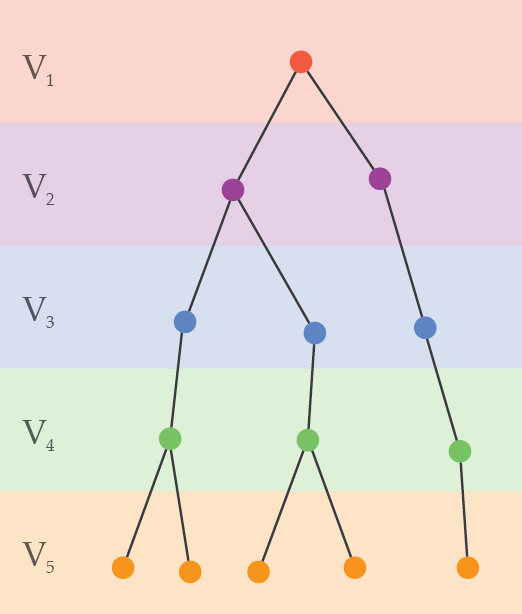
\includegraphics[width=.5\linewidth]{figures/5-tree-colour.png}} 
    \caption{An example of a balanced tree of height 4. Vertex partitions $V_1, \dots, V_5$ are coloured as described in \autoref{cor:balanced-4-tree}.}
\end{figure}

\noindent
Since paths are special cases of balanced trees, we can apply \autoref{cor:balanced-trees} to show that long paths are not levelable.

\begin{corollary} \label{cor:long-paths}
Paths on 7 or more vertices are not levelable.
\end{corollary}
\begin{proof}
Every path is also a balanced tree by taking an endpoint to be the root. There is then only one leaf (the other endpoint of the path), and therefore must be balanced. A path of length $n$ is hence a tree of height $n-1$ and by \autoref{cor:balanced-trees} is not levelable for $n \geq 7$.
\end{proof}

\section{Obstruction via graph adjoinment} \label{sec:adjoinment}

In this section we introduce a graph operation that ensures non-levelability by attaching a non-levelable graph.

\begin{definition}
If $A$ and $B$ are non-empty graphs, then $G$ is an \textbf{adjoinment} of $A$ and $B$ if $G = A\cup B \cup X$, where $X$ is a path with an endpoint in $A$ and the other in $B$. We call $X$ an \textbf{adjoining path} between $A$ and $B$. More generally, we call a graph $G$ a \textbf{$(p_1, \dots, p_k)$-adjoinment} of $A$ and $B$ if the vertex set of $G$ can be written 
\begin{equation*}
\begin{aligned}
V(G) = V(A)
\cup V(B) 
\cup V(X_1) \cup \cdots \cup V(X_k)
\end{aligned}
\end{equation*}
and the edge set 
\begin{equation*}
\begin{aligned}
E(G) =  E(A) \cup E(B) \cup E(X_1) \cup \cdots \cup E(X_k) 
\end{aligned}
\end{equation*}
where 
\begin{enumerate}
\item $V(X_i) = \br{v_{i, 1}, \dots, v_{i, p_i}}$,
\item $E(X_i) = \br{\br{v_{i, s}, v_{i, s+1}} \; | \; s = 1, \dots, p_{i} - 1 }$,
\item $V(A) \cap V(X_i) = \br{v_{i, 1}}$, and
\item $V(B) \cap V(X_i) = \br{v_{i, p_i}}$ 
\end{enumerate}
for $i = 1, \dots, k$. 
\end{definition}

\begin{figure}[!h]
    \myfloatalign
    {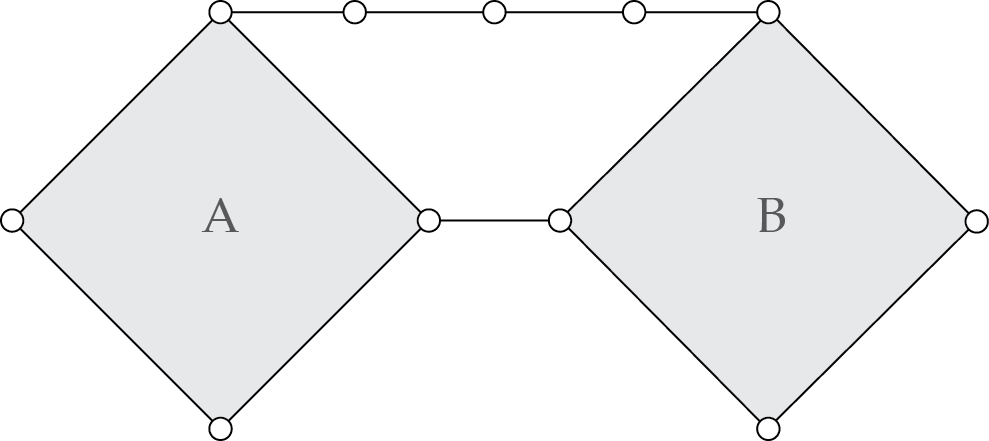
\includegraphics[width=.65\linewidth]{figures/adjoinment.png}} 
    \caption{A (5,2)-adjoinment of $A$ and $B$.}
\end{figure}

\begin{theorem}[Obstruction via adjoinment] \label{thm:adjoinment}
Let $A$ be a non-levelable graph on $V(A) = \br{v_1, \dots, v_n}$ and let $B$ be a graph on $V(B) = \br{w_1, \dots, w_m}$. Let $G$ be a $(p_1, \dots, p_k)$-adjoinment of $A$ and $B$ with $k \geq 1$ and $p_i \geq 4$ for all $i$. Then $G$ is also not levelable.
\end{theorem}

\begin{proof}
First, note that on every adjoinment path $X_i$, denote by $v_{i, 3}$ the vertex on the path that is distance 2 from $A$. Denote by $C_1, \dots, C_s$ the maximal independent sets of $A$, and let $D$ be a maximal independent set on $G \setminus A$ with $\br{v_{1,3}, \dots, v_{k,3}} \subseteq D$. To see why this is possible, note that since each path $X_i$ is on at least 4 vertices, every $v_{i,3}$ is adjacent only to $v_{i, 2}$ and $v_{i, 4}$ (and thus not adjacent to any $v_{j,3}$). 

It follows that for $i = 1, \dots, s$, $F_i = C_i \cup D$ is a maximal independent set of $G$. To check that these are independent sets, we need only check edges between $C_i$ and $D$. By construction of the adjoinment and choice of $D$, every vertex in $D$ is only connected to $A$ through some $v_{i, 3}$, and is therefore at least distance 2 from any vertex in $A$. So this is an independent set of $G$. To see that this is maximal, notice that we cannot add any vertex in $A$, since $C_i$ is maximal in $A$, and similarly we cannot add any vertex in $G \setminus A$, since $D$ is maximal in $G \setminus A$. 

Suppose then, that there exists some solution $(x_1, \dots, x_n, \dots, x_{N})$ to \autoref{thm:level-condition}, where $x_1, \dots, x_n$ correspond to the vertices in $A$. and the last $N-n$ correspond to the vertices in $G \setminus A$. The first $s-1$ equations of the system are
\begin{equation*}
S(F_i) - S(F_{i+1}) = |F_i| - |F_{i+1}|
\end{equation*}
for $i = 1, \dots, s-1$. However, given that $D$ is disjoint from each $C_i$, this is equivalent to
\begin{equation*}
S(C_i) + S(D) - S(C_{i+1}) - S(D) = |C_{i}| + |D| - |C_{i+1}| - |D|,
\end{equation*}
i.e.,
\begin{equation*}
S(C_i) - S(C_{i+1}) = |C_{i}|  - |C_{i+1}|
\end{equation*}
for $i = 1, \dots, s-1$. These equations depend only on vertices in $A$, and so if $(x_1, \dots, x_n, \dots, x_N)$ were a valid solution, then $(x_1, \dots, x_n)$ is a valid solution to these $s-1$ equations. However, this is exactly the system that needs to be satisfied in order for $A$ to be levelable, which gives a contradiction.
\end{proof}

Using the fact that the path on 5 vertices is not levelable, we can give an alternate proof for the non-levelability of cycles using \autoref{thm:adjoinment}.

\begin{corollary}
Cycle graphs on 10 or more vertices are not levelable.
\end{corollary}
\begin{proof}
Let $G = C(n)$ denote the cycle graph on $n \geq 10$ vertices. Then $G$ can expressed as a (4, 4)-adjoinment of $A$, the path graph on 5 vertices, and $B$, the path graph on $n-9$ vertices, where the adjoinment paths connect the endpoints of $A$ and $B$ to create a cycle. Since the path on 5 vertices is not levelable, applying \autoref{thm:adjoinment} tells us $G$ is not levelable.
\end{proof}

\begin{example} (The 10-cycle is not levelable). \label{ex:10-cycle}
Let $A$ denote the path on 5 vertices $\br{a_1, \dots, a_5}$ where $a_1$ and $a_5$ are the endpoints of the path, and $B$ denote the graph on 1 vertex $\br{b}$. Now, let $X_1$ be a path on 4 vertices $\br{v_{1, 1}, v_{1, 2}, v_{1,3}, v_{1,4}}$ 
where $v_{1,1}$ is a relabelling of $a_1$ and $v_{1,4}$ is a relabelling of $b$. Similarly, let $X_2$ be a path on 4 vertices $\br{v_{2, 1}, v_{2, 2}, v_{2, 3}, v_{2, 4}}$, where $v_{2, 1}$ is a relabelling of $a_5$ and $v_{2, 4}$ is a relabelling of $b$. Then $G = A\cup X_1 \cup X_2 \cup B$ is a (4, 4)-adjoinment of $A$ and $B$ (for an illustration, see \autoref{fig:10-cycle}). By \autoref{thm:adjoinment}, this graph is not levelable, since the path $A$ on 5 vertices is not levelable.

We verify this result with a specific application of the proof in \autoref{thm:adjoinment}. Notice that
\begin{equation}
\begin{aligned}
&C_1 = \br{a_1, a_3, a_5}, \\
&C_2 = \br{a_2, a_4}, \\
&C_3 = \br{a_2, a_5}, \textrm{ and }\\
&C_4 = \br{a_1, a_4}
\end{aligned}
\end{equation}
are maximal independent sets of $A$. Take $D = \br{v_{1,3}, v_{2,3}}$. Then $F_i = C_i \cup D$ is a maximal independent set of $G$ for $i = 1, \dots, 4$. Consider some potential solution $(a_1, \dots, a_5, b, v_{1,2}, v_{1,3}, v_{2, 2}, v_{2, 3})$. Notice that for any $S(F_i) - S(F_{i+1}) = |F_i| - |F_{i+1}|$, we can write this as 
\begin{equation}
\begin{aligned}
S(C_i) + S(D) - S(C_{i+1}) - S(D) = |C_i| + |D| - |C_{i+1}|- |D| 
\end{aligned}
\end{equation}
i.e., $S(C_i) - S(C_{i+1}) = |C_i| - |C_{i+1}|$. These equations depend only on vertices in $A$, and do not have a valid solution since the path on 5 vertices is not levelable.

\end{example}
\begin{figure}[bth]
    \myfloatalign
    \subfloat
    {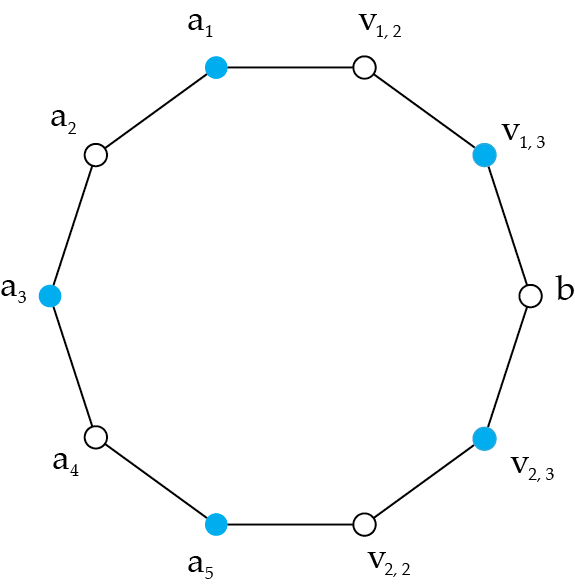
\includegraphics[width=.4\linewidth]{figures/cycle-adjoinment-1.png}} \qquad 
    \subfloat
    {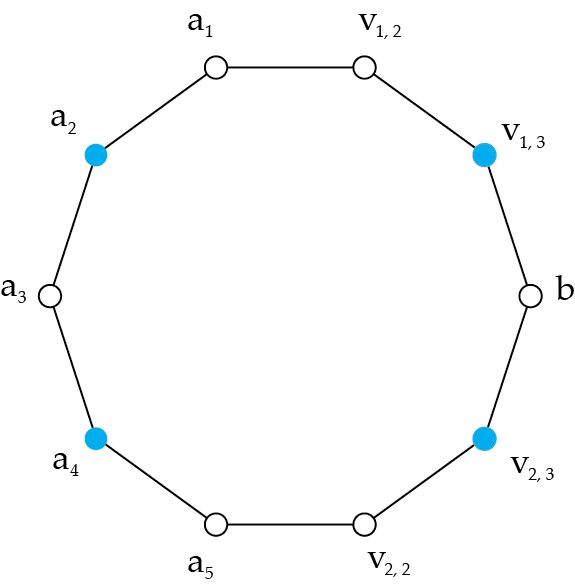
\includegraphics[width=.4\linewidth]{figures/cycle-adjoinment-2.png}} \\
    \subfloat
    {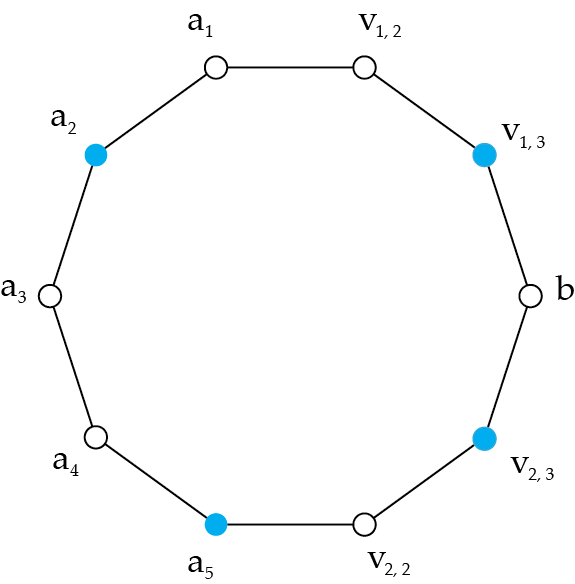
\includegraphics[width=.4\linewidth]{figures/cycle-adjoinment-3.png}} \qquad
    \subfloat
    {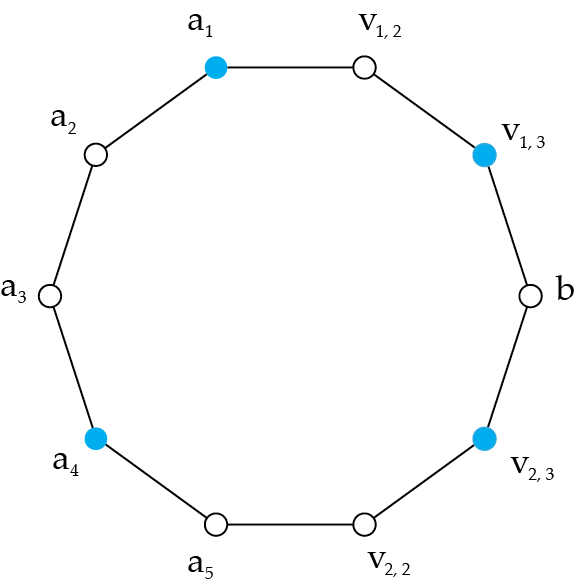
\includegraphics[width=.4\linewidth]{figures/cycle-adjoinment-4.png}}
    \caption{The cycle on 10 vertices labelled as a (4, 4)-adjoinment between the path on 5 vertices and the graph on 1 vertex as described in \autoref{ex:10-cycle}. Facets are shown in blue. Notice that the independent set $D = \br{v_{1, 3}, v_{2, 3}}$ is contained in every facet.} \label{fig:10-cycle}
\end{figure}

\section{Adding vertices} \label{sec:adding-vertices-non-levelable}
In \autoref{sec:adding-vertices-levelable}, we showed that adding vertices (up to some limit) preserves the levelability of a graph. In this section, we show a similar statement for non-levelable graphs. That is, adding vertices to a non-levelable graph will yield a non-levelable graph.

\begin{theorem} \label{thm:adding-vertices-non-levelable}
Let $G$ be a non-levelable graph with vertex set $V(G) = \br{v_1, \dots, v_n}$, and let $F_1, \dots, F_t$ denote the facets of $\ind(G)$. Define $G'$ to be the graph with vertex $V(G') = V(G) \cup \br{w_1, \dots, w_m}$ for some $m \in \mathbb{N}$ and edge set $E(G')$ such that:
\begin{enumerate}
\item $E(G) \subset E(G')$, and 
\item $N(F_i) \cap \br{w_j} \neq \emptyset$ for $i = 1, \dots, t$, $j = 1, \dots, m$.
\end{enumerate}
Then $G'$ is not levelable.
\end{theorem}

\begin{proof}
Let $F_1, \dots, F_t$ denote the facets of $\ind (G)$. Notice that $F_1, \dots, F_t$ are also facets of $\ind (G')$, since the each of the new vertices $\br{w_1, \dots, w_m}$ is adjacent to some vertex in each $F_i$, and so they cannot be added to any of the original facets $F_i$. 

Now, in order for $G'$ to be levelable, there must exist some solution $(v_1, \dots, v_n, \allowbreak w_1, \dots, w_m)$ to the system of equations
$$
S(F_i) - S(F_{i+1}) = |F_i| - |F_{i+1}| 
$$
for $i = 1, \dots, t'$, where $t'>t$ is the number of facets of $\ind (G')$. However, notice that the first $t-1$ equations concern the $t$ facets from $G$, and depend only on vertices from $V(G)$. If some $(v_1, \dots, v_n, \allowbreak w_1, \dots, w_m)$ was a valid solution to the $t$ equations, then $(v_1, \dots, v_n)$ must be a valid solution to the $t-1$ equations for $G$. Hence $G$ must have been levelable, giving a contradiction. Thus $G'$ is not levelable. 
\end{proof}

It is interesting to consider the converse of this statement. That is, for a non-levelable graph $G$ such that some vertex $\br{v'}$ is adjacent to all the maximal independent sets of $G$, is the induced subgraph $G'$ with $V(G') = V(G) \setminus \br{v'}$ also non-levelable? formally state this quesiton in \autoref{sec:question-adding-non}.

We can apply this result to generalize our observation regarding wheel graphs in \autoref{subsec:cycles-wheels}. 

\begin{corollary}
The wheel graph on $n+1$ vertices is levelable if and only if the cycle on $n$ vertices is levelable.
\end{corollary}

\begin{proof}
This is just an application of \autoref{thm:adding-vertices-non-levelable}. Adding a completely connected vertex to the cycle graph on $n$ vertices produces the wheel graph on $n+1$ vertices.
\end{proof} % Chapter 3
\include{Chapters/not-levelable-results} % Chapter 4 
\changelocaltocdepth{0}

\chapter{Open Questions and Conjectures}
\label{ch:conjectures}

This chapter summarizes some open questions and conjectures arising from the computer search and findings in the previous chapters.

\section{Enumeration of levelable graphs} In \autoref{sec:enumeration} we presented a table showing the number of levelable graphs on $n \leq 10$ vertices. For larger graphs, checking the levelable condition becomes computationally burdensome due to the large linear system and the number of connected graphs. It remains an open question how the number of levelable graphs grows with the number of vertices.

\begin{question}
For $n > 10$, how many graphs on $n$ vertices are levelable?
\end{question}

\section{Caterpillar Graphs} In \autoref{sec:caterpillar}, we introduced caterpillar graphs, which are special tree graphs where all vertices are at most distance 1 from a central path. In \autoref{thm:caterpillar} we showed that if every vertex on the central path contains at least one ``leg'' vertex, then the graph most be levelable. The data generated from the computer search suggest that this is also a necessary condition, since all levelable caterpillars on 10 or fewer vertices satisfy this ``minimum leg condition.'' We therefore state the converse statement of \autoref{thm:caterpillar} as the following conjecture:

\begin{conjecture}
A caterpillar graph $G$ is levelable if and only if every vertex on the central path (except for perhaps the endpoints of the path) has at least one leg vertex. 
\end{conjecture}

\section{Graph Expansions}
First, recall from \autoref{thm:expansion} that performing a uniform graph expansion on a levelable graph produces a new levelable graph. That is, the levelablity of a graph is preserved if we replace each vertex with an independent set of some size $k \geq 1$. However, we have not yet addressed a general graph expansion on $G$ where the $n$ vertices $V(G) = \br{v_1, \dots, v_n}$ are replaced with independent sets of size $k_1, \dots, k_n$ respectively. Are there weaker conditions on $k_1, \dots, k_n$ or the graph $G$ that still preserves the levelability of a graph? In other words:

\begin{question}
For a levelable graph $G$, under what conditions is a non-uniform expansion of $G$ also levelable?
\end{question}

\section{Adding vertices to levelable graphs} In \autoref{sec:adding-vertices-levelable}, we proved that given a levelable graph $G$ with maximal independent sets $F_1, \dots, F_t$, we can construct a new levelable graph by adding $m \leq \max\br{|F_i|}$ new vertices adjacent to all existing vertices. However, this bound on $m$ arose out of convenience with respect to the system in \autoref{thm:level-condition}. Therefore, it is likely there are cases in which we can relax this bound, which raises the following question:

\begin{question}
For a levelable graph $G$ with maximal independent sets $F_1, \dots, F_t$, under what conditions does adding $m > \max\br{|F_i|}$ completely connected vertices produce a levelable graph?
\end{question}

\section{Adding vertices to non-levelable graphs} \label{sec:question-adding-non} \autoref{thm:adding-vertices-non-levelable} states that adding vertices that are adjacent to at least one vertex in each facet of a non-levelable graph yields a new non-levelable graph. Is the converse statement true? We pose this as an open question:
\begin{question}
Let $G$ be a non-levelable graph with a vertex $v'$ such that $v'$ is adjacent to all maximal independent sets of $G$. Let $G'$ denote the induced subgraph $G'$ with $V(G') = V(G) \setminus \br{v'}$ and $E(G') = E(G) \setminus \br{\br{v', w} \; | \; \br{v', w} \in E(G)}$. Is $G'$ also non-levelable?
\end{question}

In this report we have also explored cases in which the addition of vertices does not satisfy the condition in \autoref{thm:adding-vertices-non-levelable} but still results in a non-levelable graph (e.g. adding a vertex to the 5-path to create the 6-path). There are also cases where the resulting graph is levelable (e.g. the graph in \autoref{ex:5-path-induce}, where one vertex was added to the path to create a 3-cycle). It is therefore an interesting problem to relax this condition for \autoref{thm:adding-vertices-non-levelable}, as well as identify where we can add vertices to make a non-levelable path graph levelable.
\begin{question}
If $G$ is the path graph on $n$ vertices, where must vertices and edges be added to make the resulting graph levelable?
\end{question}
\noindent
More generally, we ask:
\begin{question}
If $G$ is a non-levelable graph, what graph operations make the resulting graph levelable?
\end{question}

\section{Other criteria on vertex partitions} \label{sec:other-criteria}
In \autoref{thm:graph-partitions}, we showed that we can preclude levelability if the vertex set of a graph can be partitioned in a certain way such that certain unions of the partitioning sets are maximal independent sets. This criterion was based on the independent sets of the path on 5 vertices. In \autoref{ex:5-path} we formally showed the non-existence of a valid solution to the system for the path on 5 vertices, and the proof \autoref{thm:graph-partitions} depended on a similar contradiction. In the latter, the partition sets of the vertex set ``represented" the vertices of the path. Can we exploit the independent set structure of other non-levelable to construct new criteria in a similar way to \autoref{thm:graph-partitions}? We leave this as an open problem: 
\begin{question} 
Do there exist other paritions of $V(G)$ similar to \autoref{thm:graph-partitions} that prevent a graph from being levelable?
\end{question}
\noindent
We can think of the 5-path as being the ``minimal" case of \autoref{thm:graph-partitions}, since this is the case where each partition set contains only one vertex. Since the path on 6 vertices cannot be partitioned to satisfy \autoref{thm:graph-partitions}, we expect that this will yield a different partition condition. However, the paths on 7 vertices or greater are covered by the condition in \autoref{thm:graph-partitions} arising from the 5-path. We can therefore see that there is some minimal set of non-levelable graphs that give rise to a unique set of conditions that preclude levelability. 

For example, for graphs on 5 vertices, this set is trivial since there is only one non-levelable graph. Hence the path on 5 vertices gives a condition that trivially captures all non-levelable graphs on 5 vertices. However, for 6 vertices we need at least two unique conditions. The non-levelable graph $G$ on 6 vertices $V(G) = \br{v_1, \dots, v_6}$ and edge set 
$$
E(G) = \br{\br{v_i, v_{i+1}} \; | \; i = 1, \dots, 4} \cup \br{\br{v_4, v_6}}
$$
can be partitioned according to \autoref{thm:graph-partitions} (see \autoref{fig:6-vertex}), while the (non-levelable) path on 6 vertices is the minimal case of a new condition. 

\begin{figure}[bth]
    \myfloatalign
    \subfloat
    {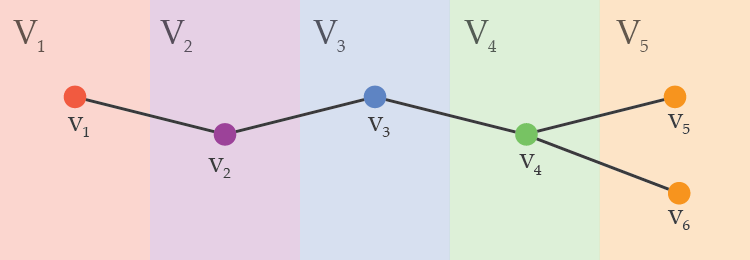
\includegraphics[width=.7\linewidth]{figures/6-vertex-1.png}} \\ \vspace{1cm}
    \subfloat
    {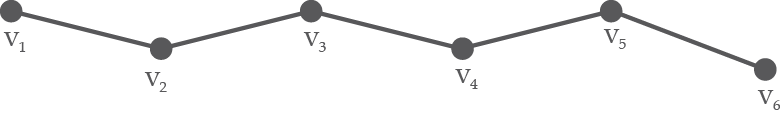
\includegraphics[width=.7\linewidth]{figures/6-path.png}} 
    \caption{An example of a graph on 6 vertices (top) that satisfies \autoref{thm:graph-partitions}, with the vertices coloured to illustrate the partition; and the path on 6 vertices (bottom), which cannot be partitioned in this way.} \label{fig:6-vertex}
\end{figure}
\noindent
This observation raises the following question:
\begin{question}
How many unique partition conditions are required to capture all non-levelable graphs on $n$ vertices?
\end{question}





\cleardoublepage % Empty page before the start of the next part

%----------------------------------------------------------------------------------------
%	THESIS CONTENT - APPENDICES
%----------------------------------------------------------------------------------------

\appendix


\chapter{Appendix: Atlas of Levelable Graphs} \label{appendix}

\section*{Non-levelable graphs on 6 vertices}

\begin{figure}[h!]
    {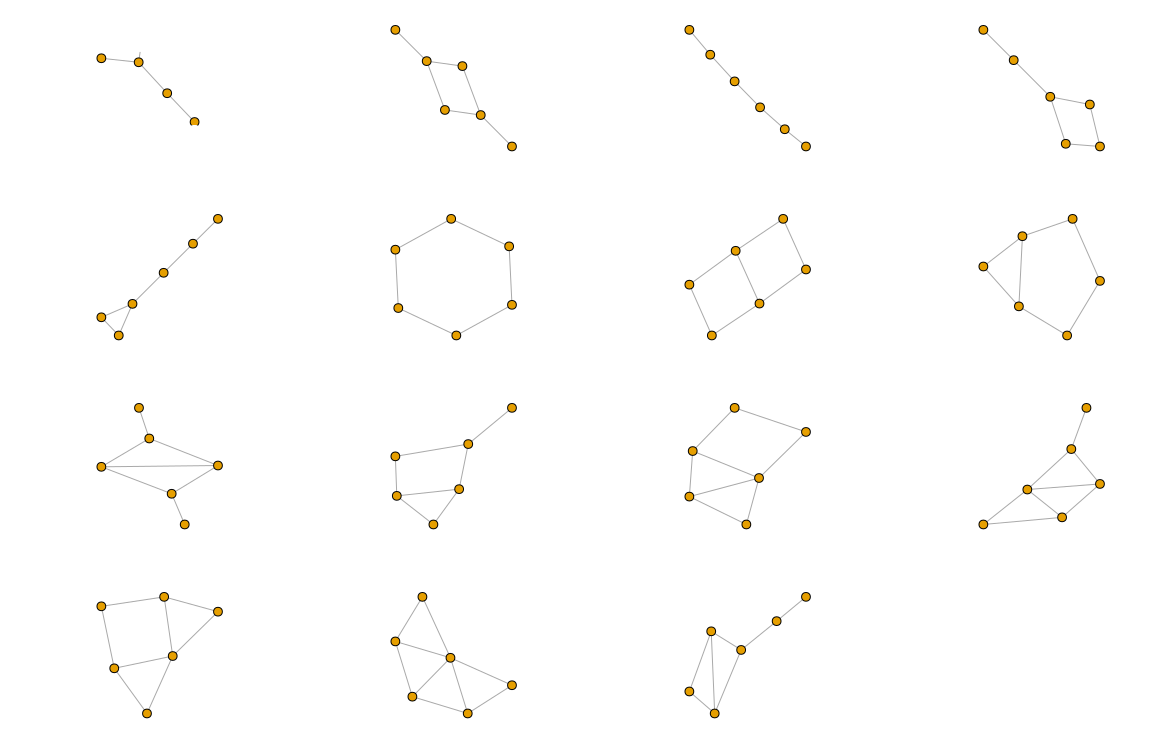
\includegraphics[width=1\linewidth]{atlas/atlas6.png}} 
\end{figure}

\section*{Non-levelable graphs on 7 vertices}
\vspace{-0.5cm}
\begin{figure}[h!]
    {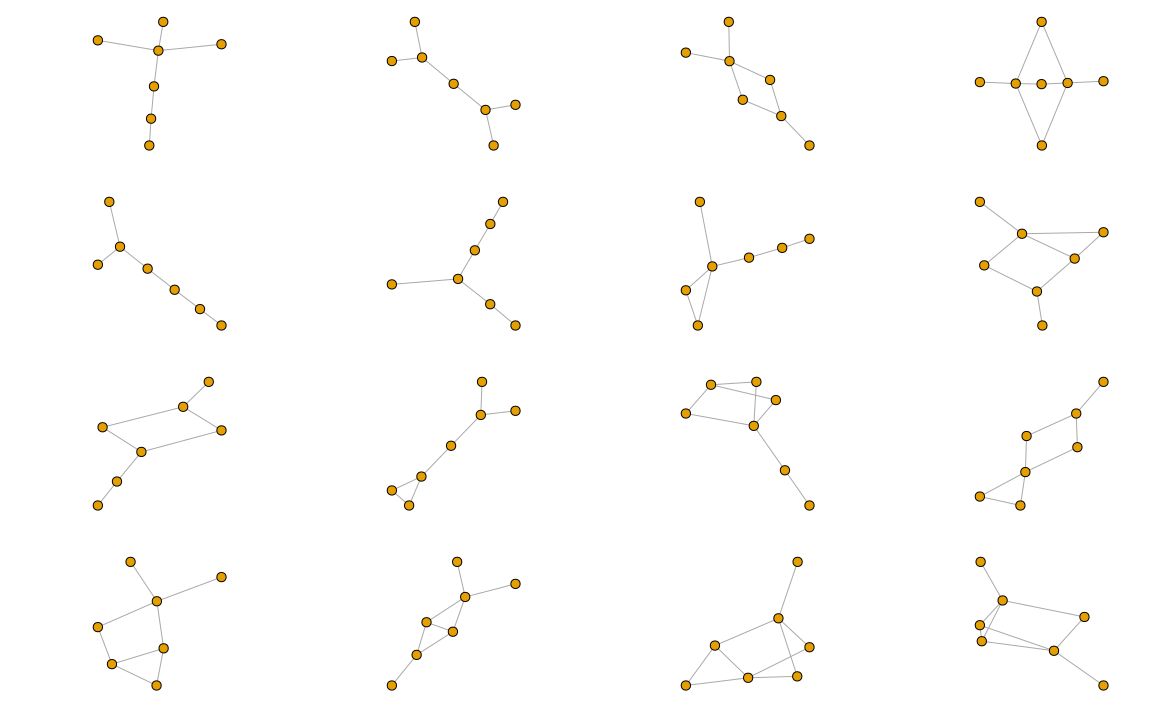
\includegraphics[width=0.95\linewidth]{atlas/atlas7-1.png}} 
\end{figure}

\begin{figure}[h!]
	\subfloat
    {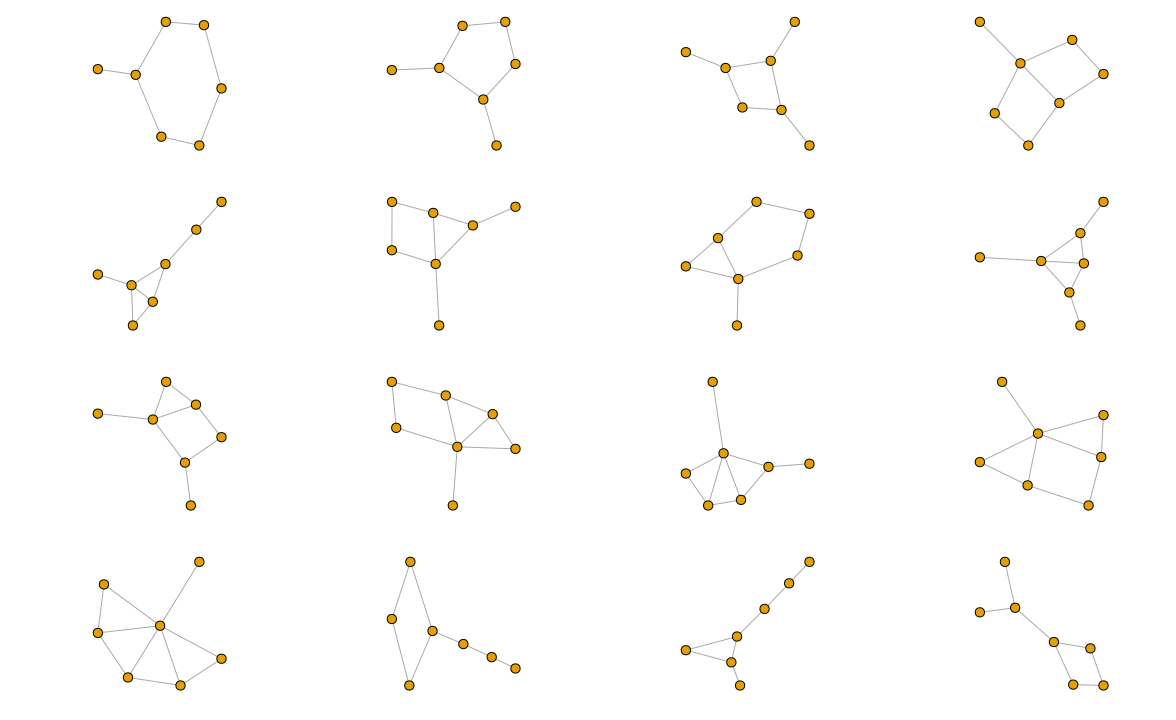
\includegraphics[width=0.95\linewidth]{atlas/atlas7-2.png}} \\
    \subfloat
    {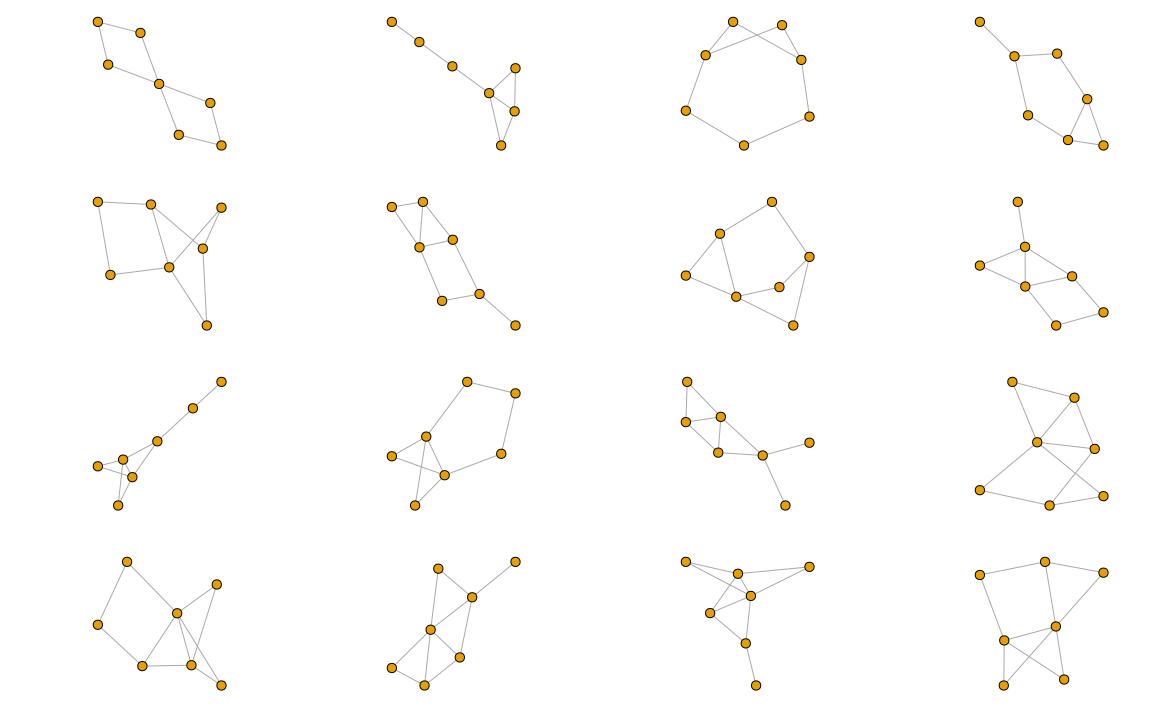
\includegraphics[width=0.95\linewidth]{atlas/atlas7-3.png}} \\
	\subfloat
    {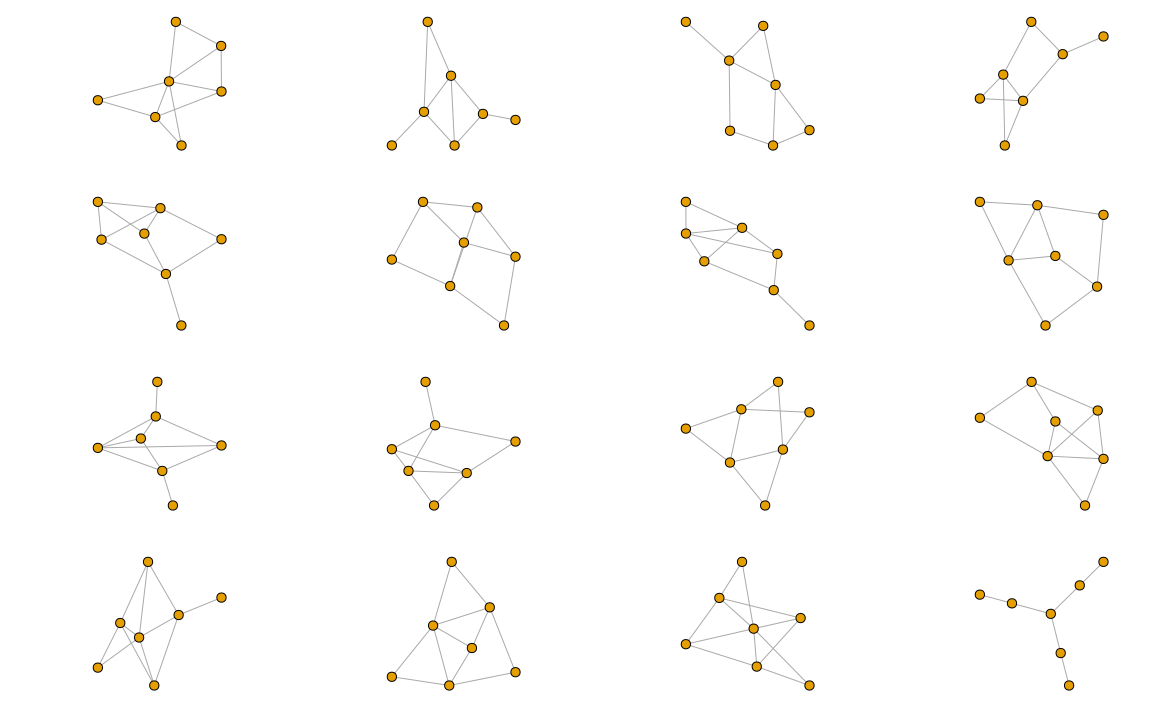
\includegraphics[width=0.95\linewidth]{atlas/atlas7-4.png}} 
\end{figure}

\begin{figure}[h!]
    \subfloat
    {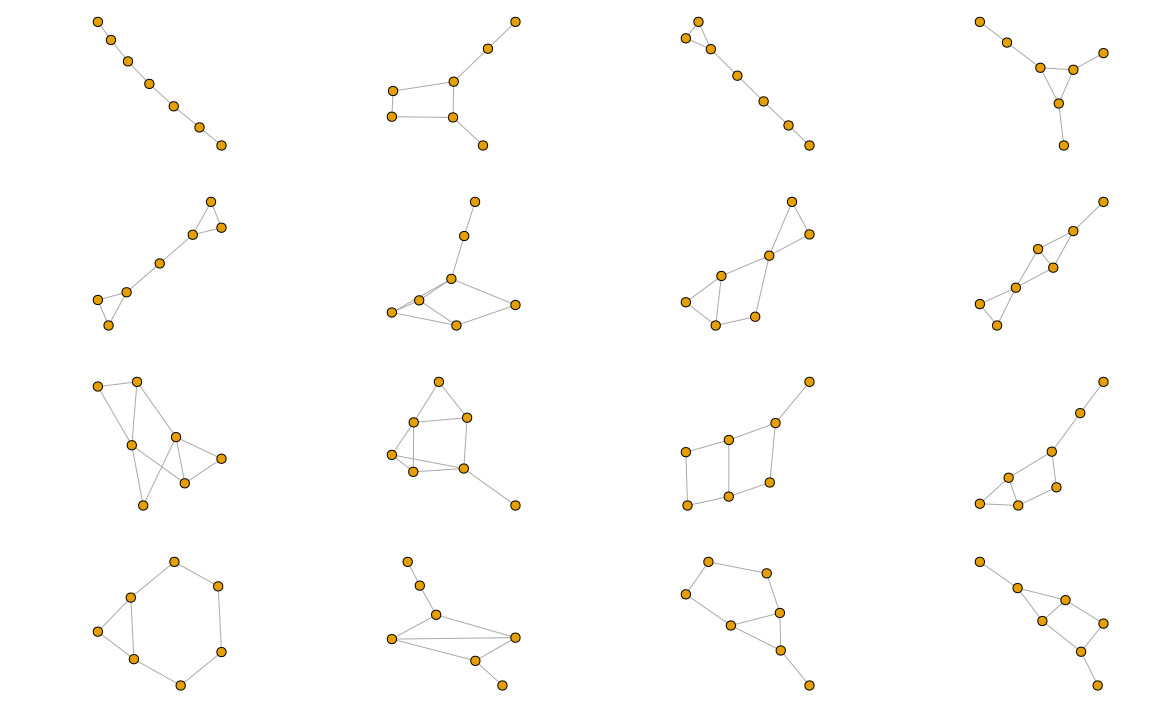
\includegraphics[width=0.95\linewidth]{atlas/atlas7-5.png}} \\
	\subfloat
    {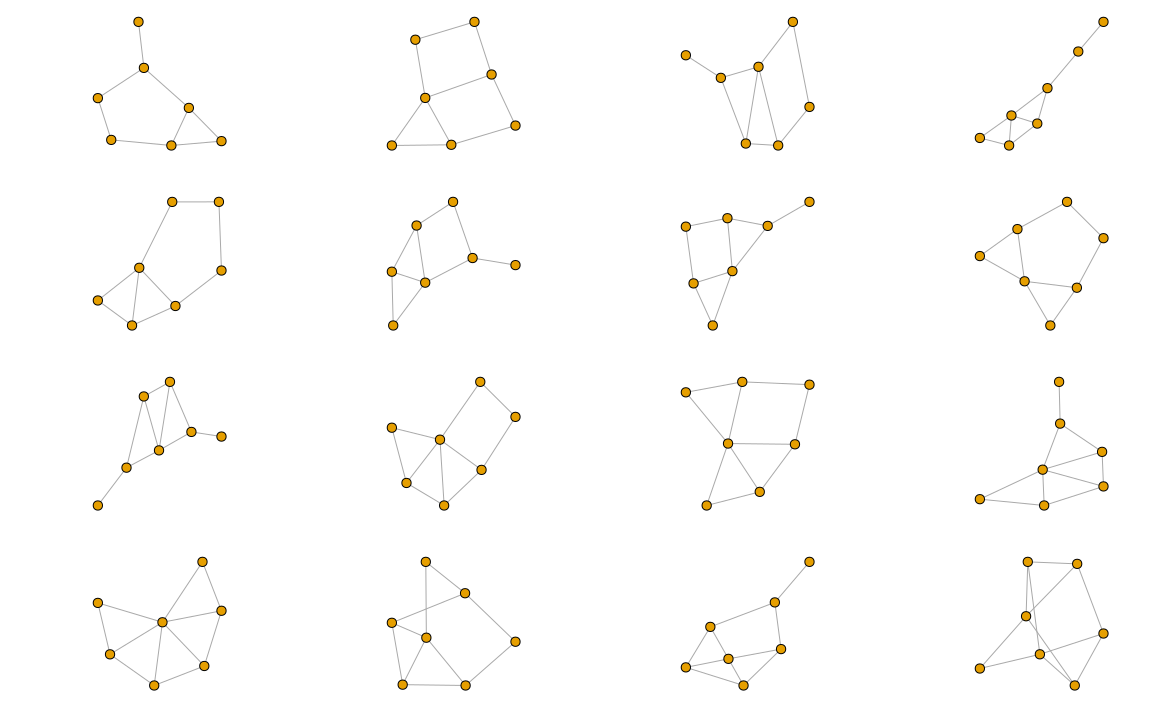
\includegraphics[width=0.95\linewidth]{atlas/atlas7-6.png}} \\
	\subfloat
    {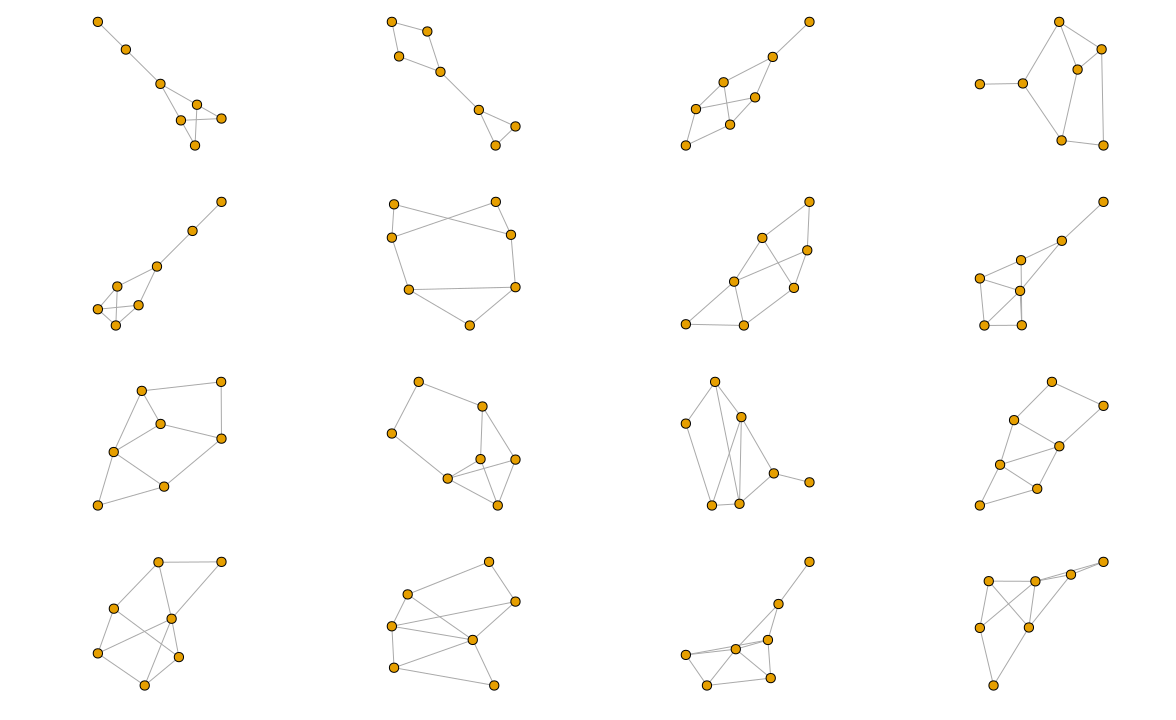
\includegraphics[width=0.95\linewidth]{atlas/atlas7-7.png}} 
\end{figure}

\begin{figure}[h!]
	\subfloat
	{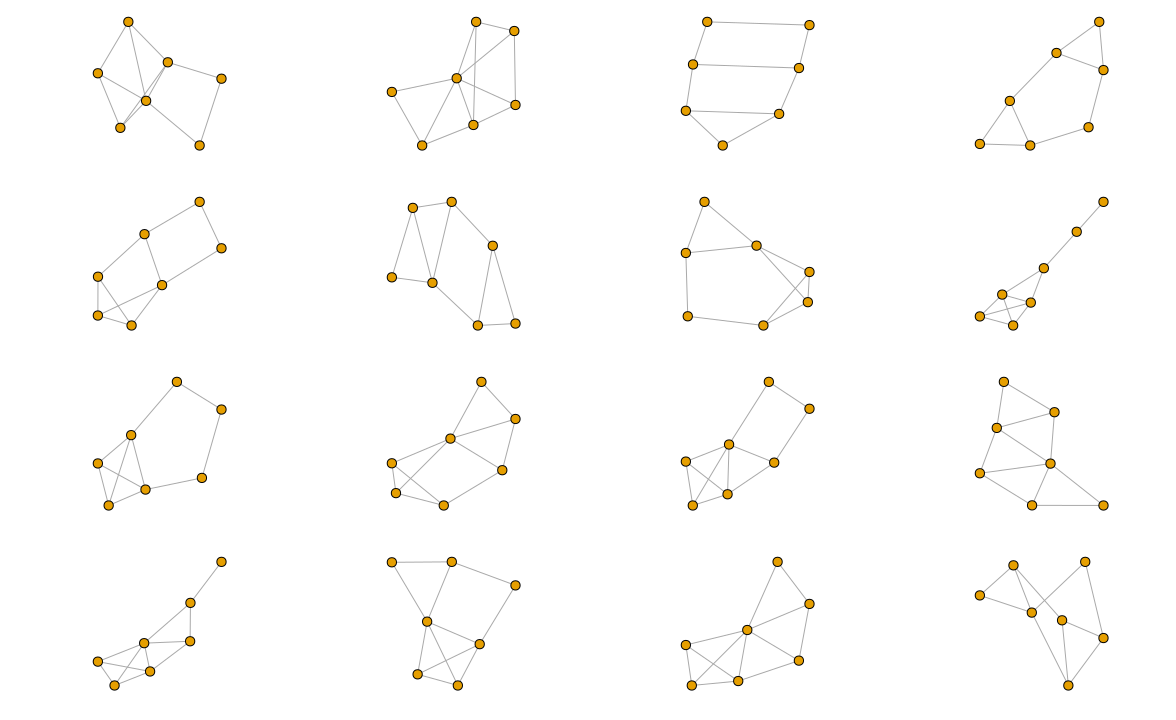
\includegraphics[width=0.95\linewidth]{atlas/atlas7-8.png}} \\
	\subfloat
    {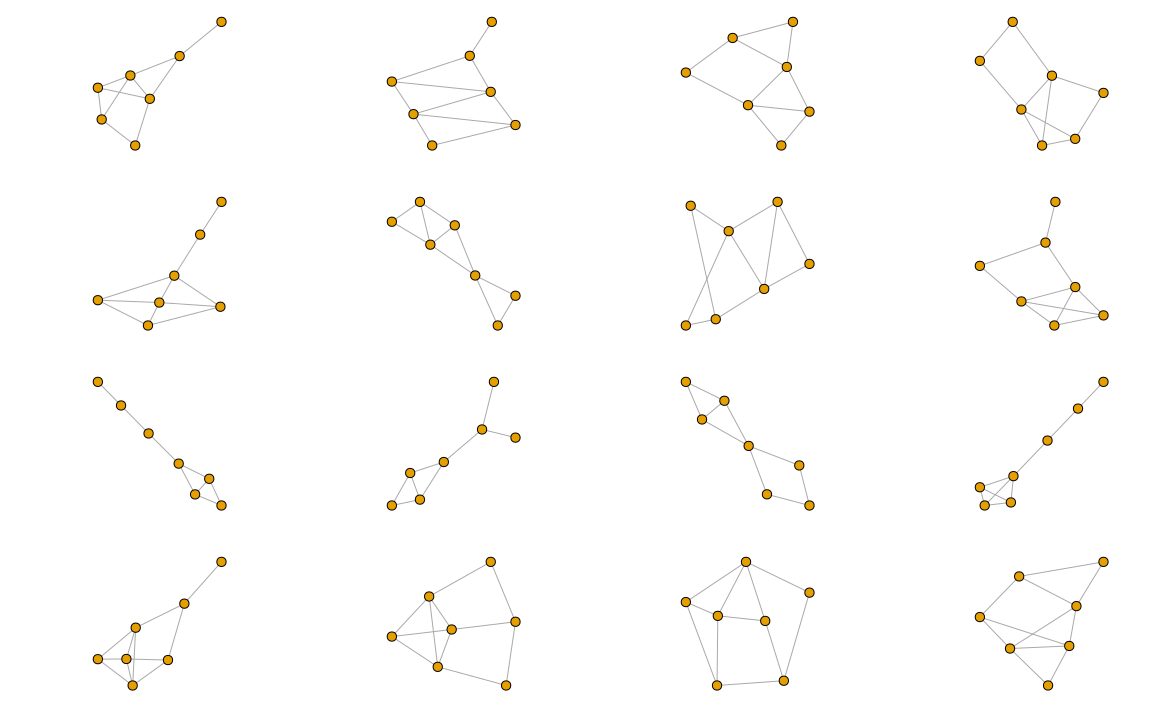
\includegraphics[width=0.95\linewidth]{atlas/atlas7-9.png}} \\
    \subfloat
    {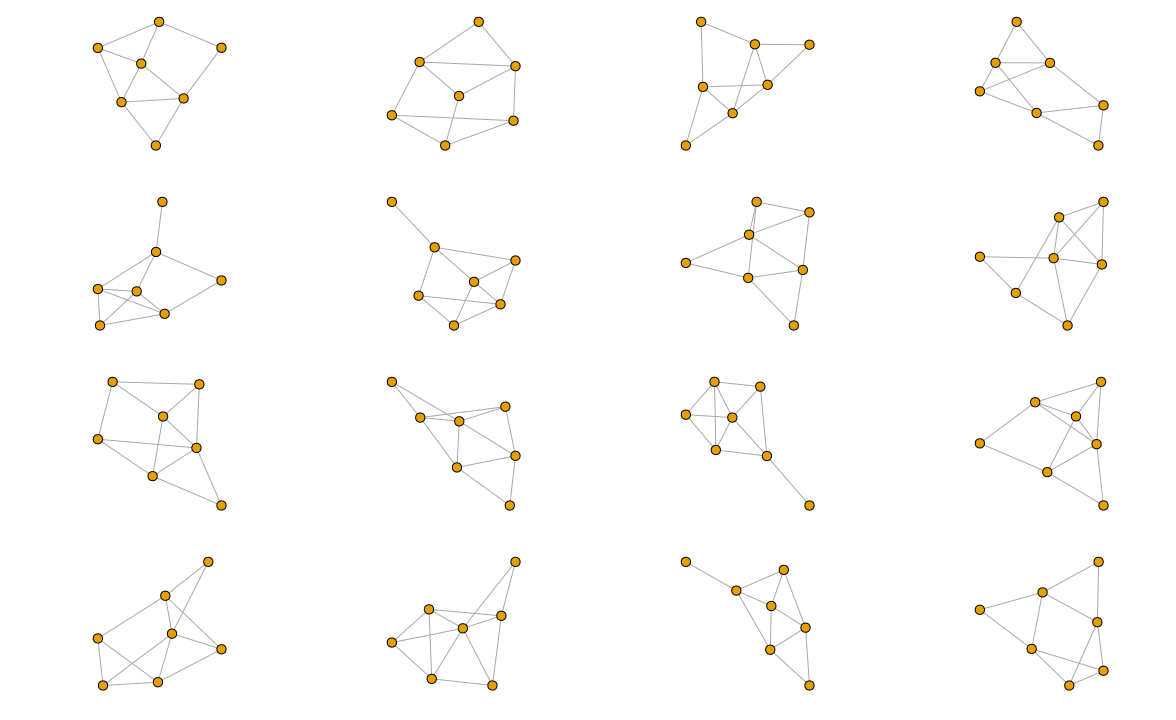
\includegraphics[width=0.95\linewidth]{atlas/atlas7-10.png}}
\end{figure}

\begin{figure}[h!]
	\subfloat
	{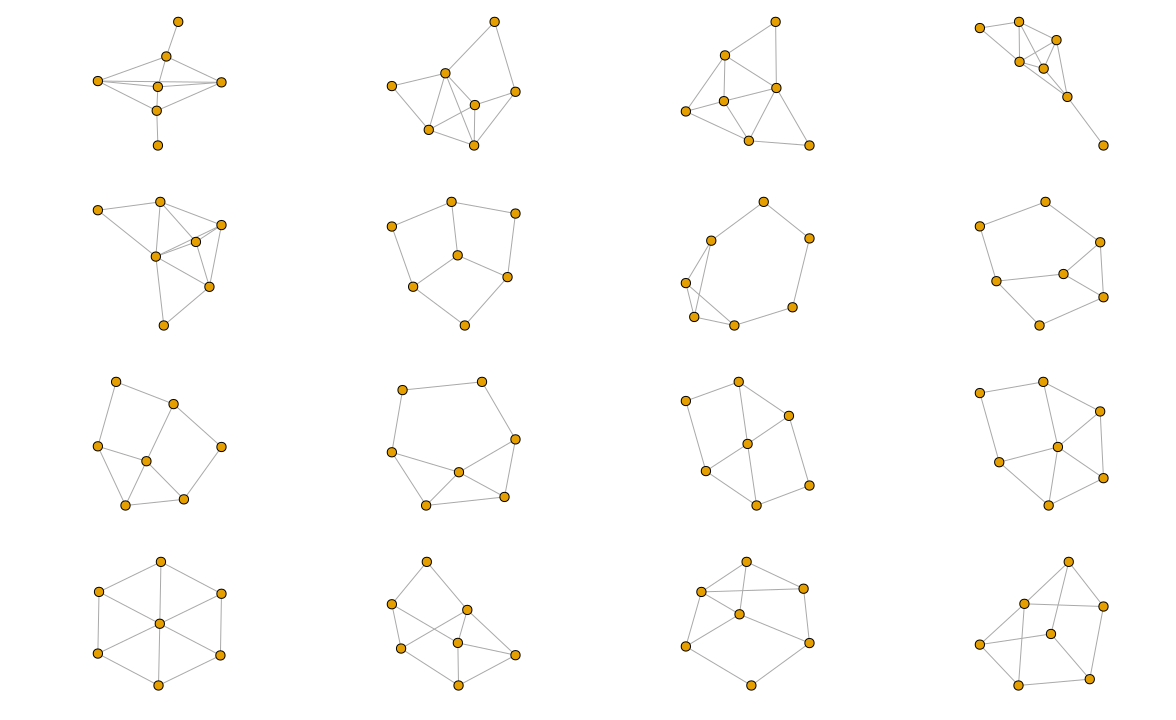
\includegraphics[width=0.95\linewidth]{atlas/atlas7-11.png}} \\
	\subfloat
    {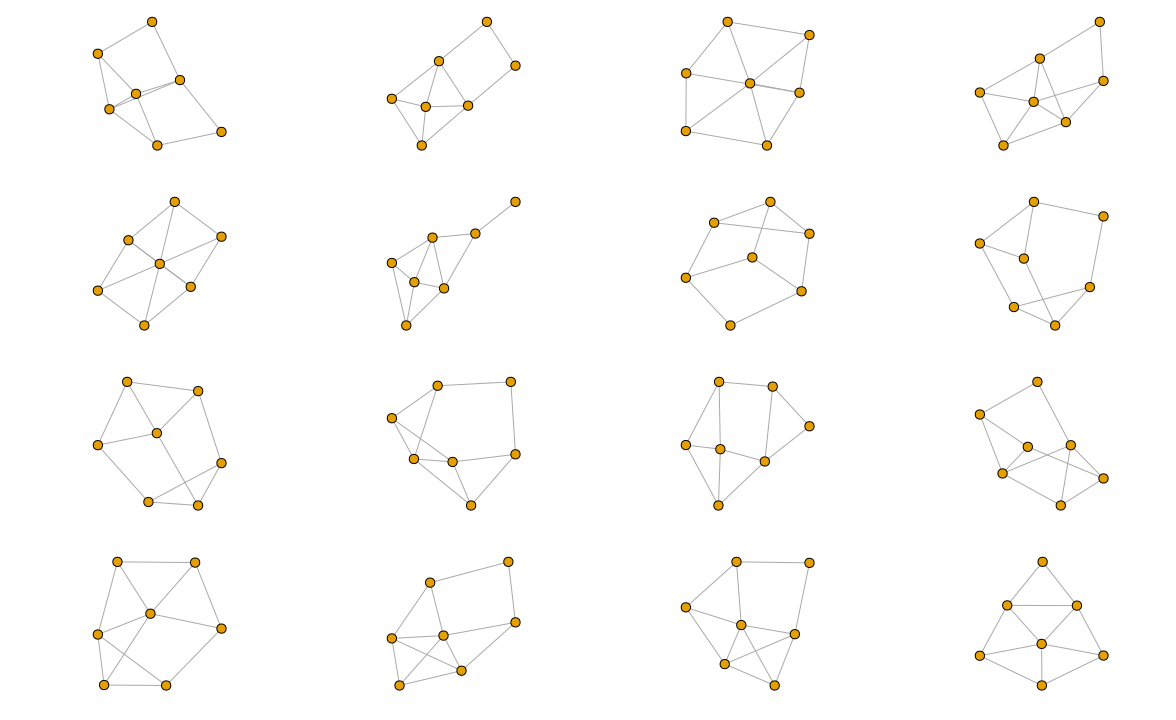
\includegraphics[width=0.95\linewidth]{atlas/atlas7-12.png}} \\
    \subfloat
    {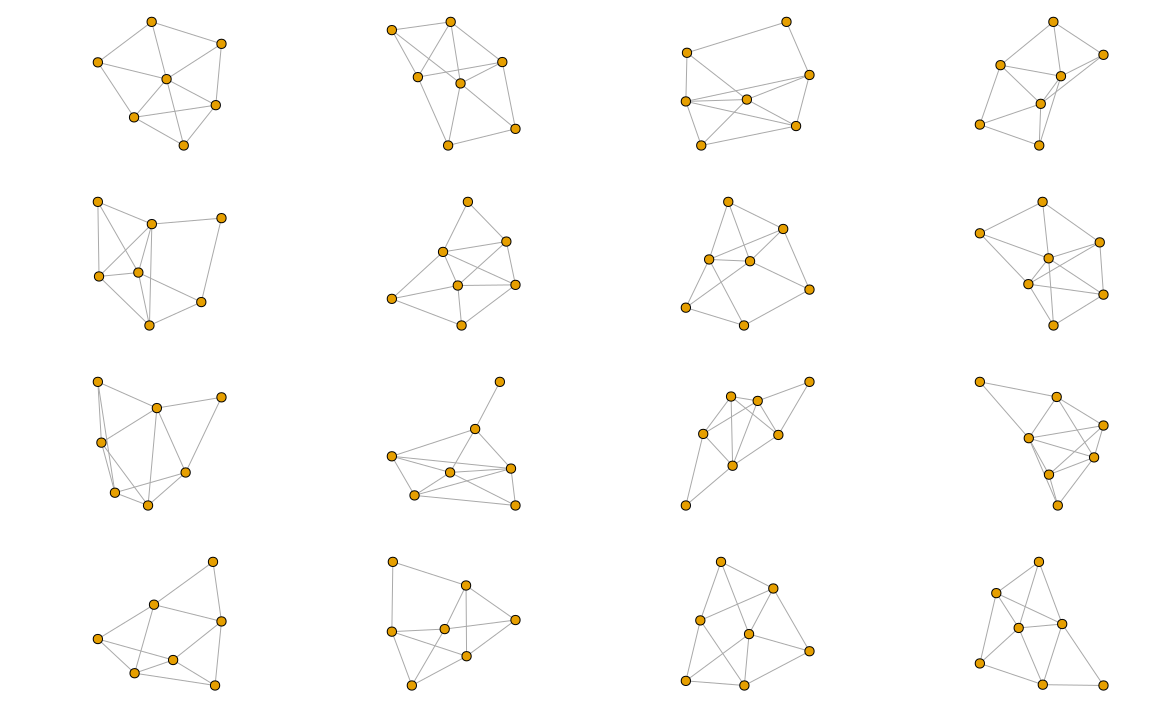
\includegraphics[width=0.95\linewidth]{atlas/atlas7-13.png}}
\end{figure}

\begin{figure}[h!]
	\subfloat
	{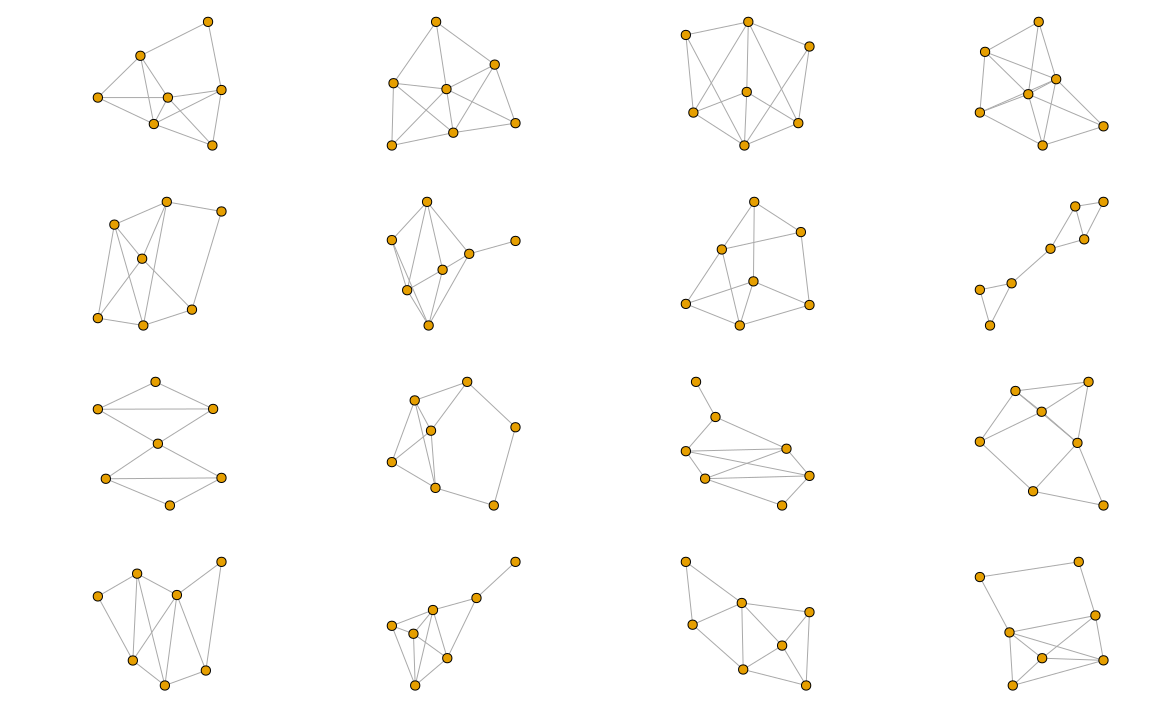
\includegraphics[width=0.95\linewidth]{atlas/atlas7-14.png}} \\
	\subfloat
    {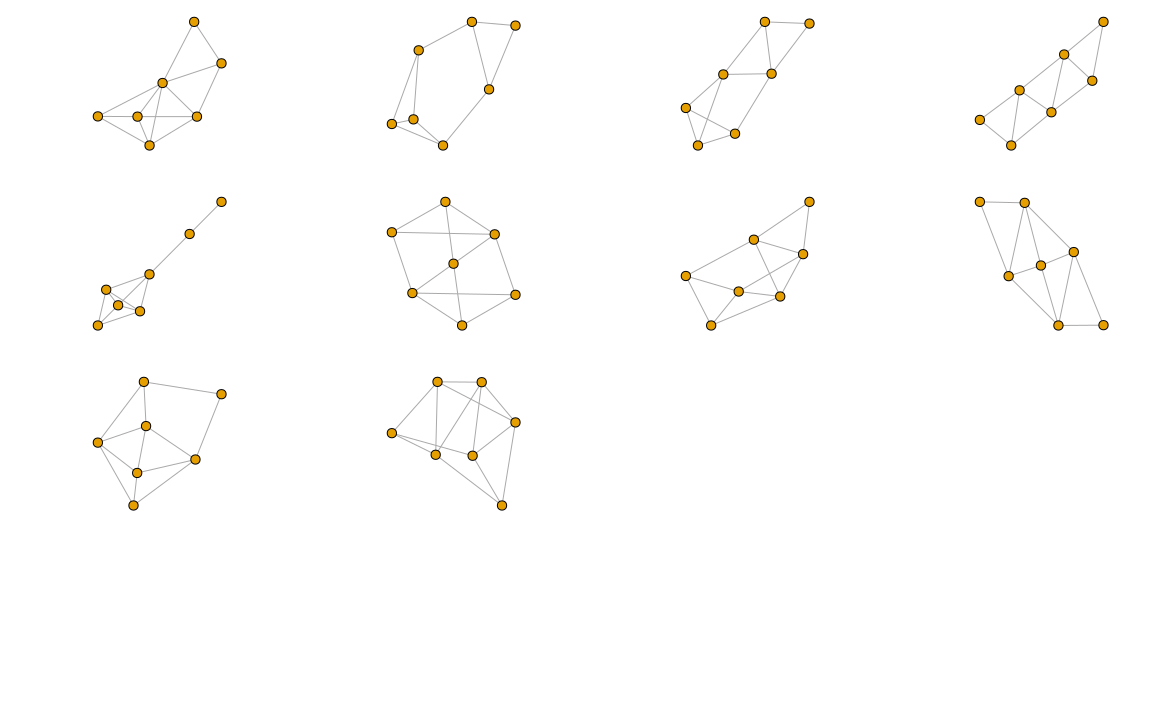
\includegraphics[width=0.95\linewidth]{atlas/atlas7-15.png}}
\end{figure} % Appendix A
%\include{Chapters/Chapter0B} % Appendix B - empty template

%----------------------------------------------------------------------------------------
%	POST-CONTENT THESIS PAGES
%----------------------------------------------------------------------------------------

\cleardoublepage% Bibliography

\label{app:bibliography} % Reference the bibliography elsewhere with \autoref{app:bibliography}

\manualmark % Work-around to have small caps also here in the headline
\markboth{\spacedlowsmallcaps{\bibname}}{\spacedlowsmallcaps{\bibname}} % Work-around to have small caps also
%\phantomsection
\refstepcounter{dummy}

\addtocontents{toc}{\protect\vspace{\beforebibskip}} % Place the bibliography slightly below the rest of the document content in the table of contents
\addcontentsline{toc}{chapter}{\tocEntry{\bibname}}

\printbibliography % Bibliography

% \cleardoublepage\include{FrontBackMatter/Declaration} % Declaration

%\cleardoublepage\include{FrontBackMatter/Colophon} % Colophon

%----------------------------------------------------------------------------------------

\end{document}
